\documentclass[a4paper, 10pt]{article}
% All LaTeX documents including
% tikz() output must use this
% package!
\usepackage[margin=2.5cm]{geometry}
\usepackage{tikz}
\usepackage{pdflscape}

\newcommand{\insertplot}[2]{
  \begin{figure}[!ht]
    \centering
    \input{#1}
    \caption{#2}
  \end{figure}
}

\begin{document}

% \begin{landscape}
%   \begin{figure}[!h]
%     \centering
%     % Created by tikzDevice version 0.9 on 2016-01-03 23:11:33
% !TEX encoding = UTF-8 Unicode
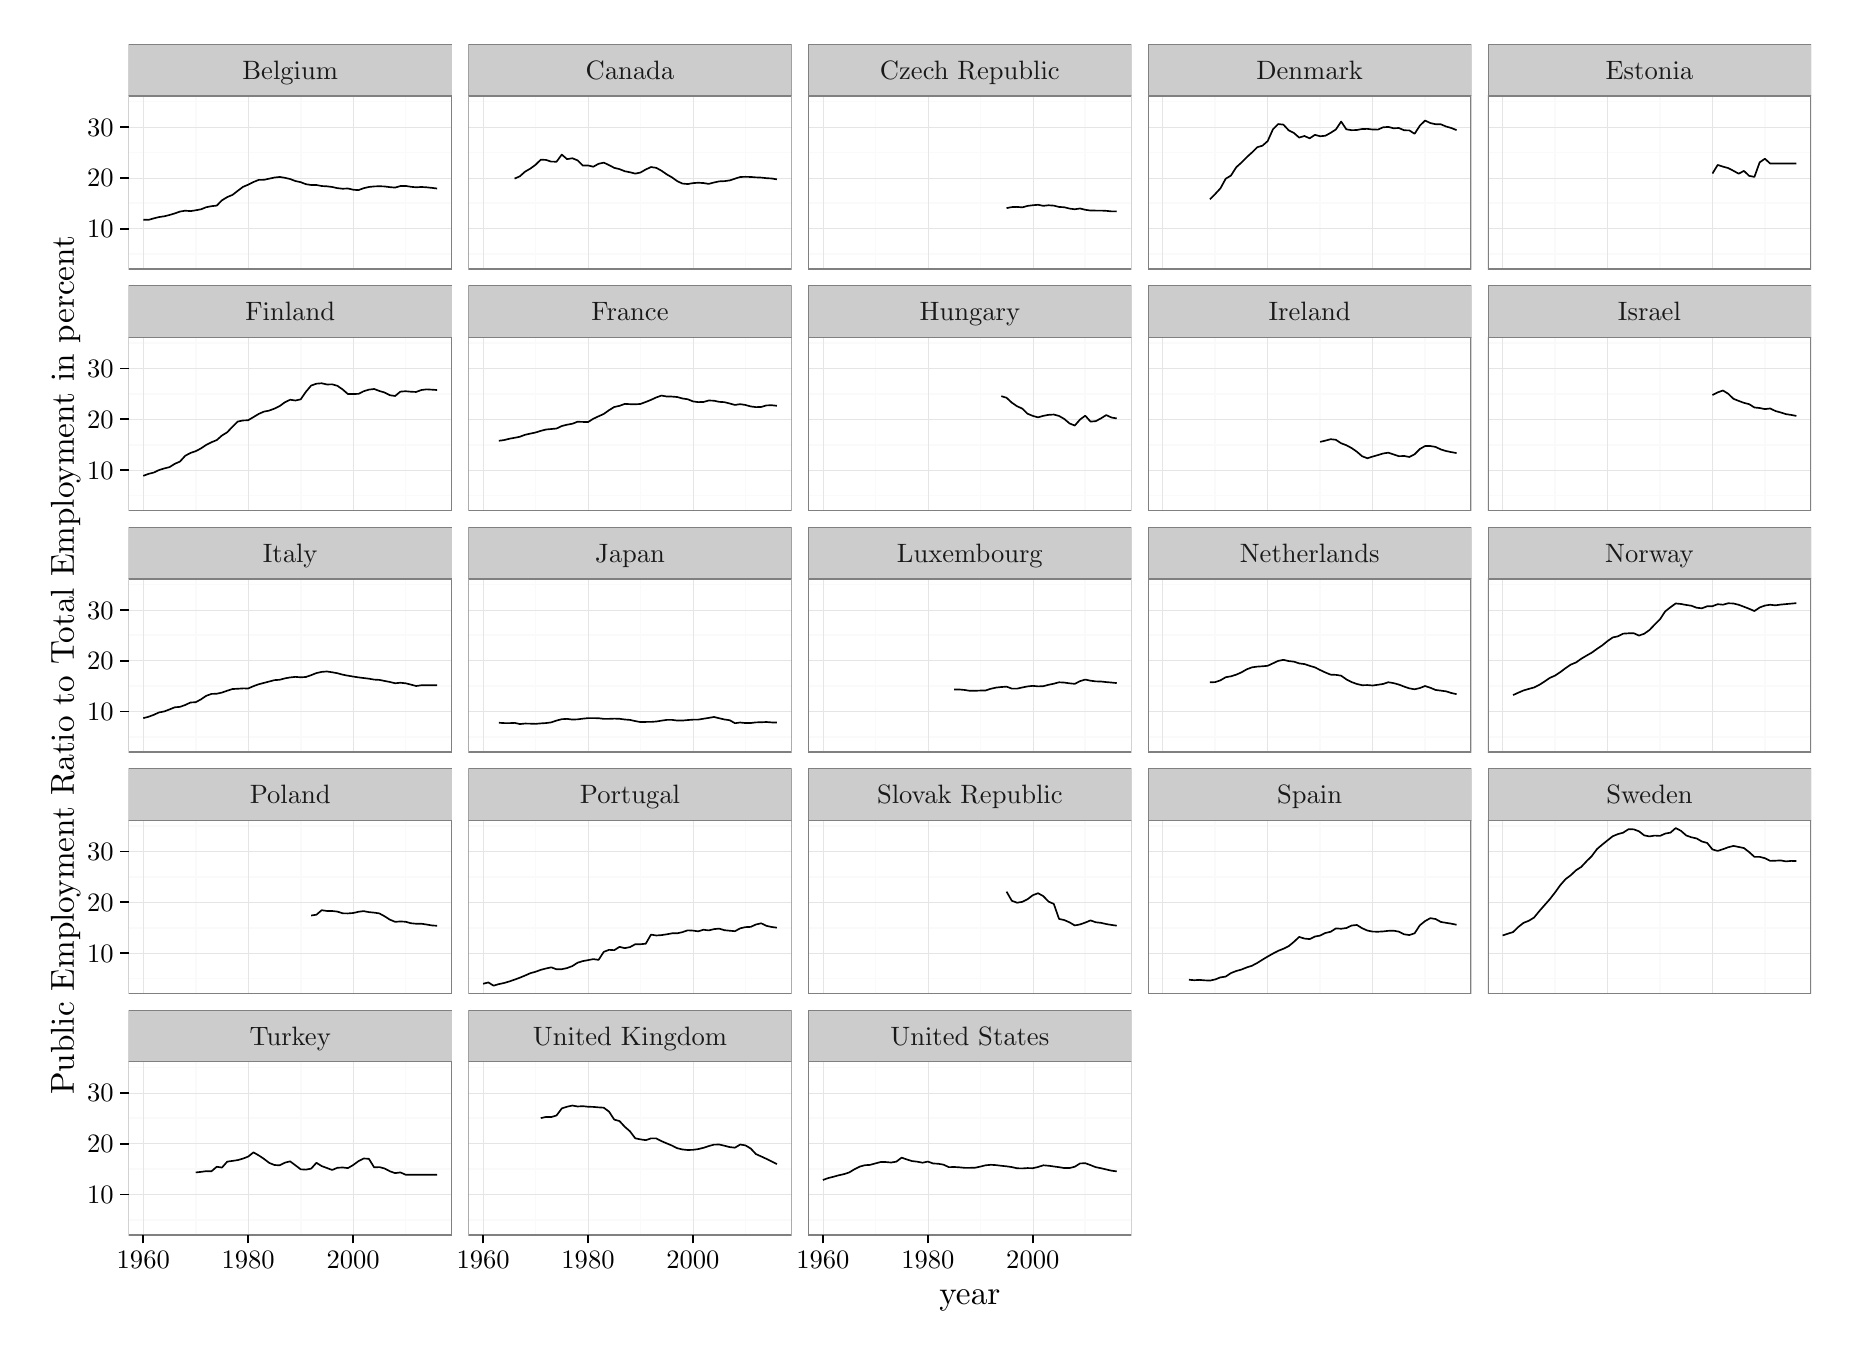
\begin{tikzpicture}[x=1pt,y=1pt]
\definecolor{fillColor}{RGB}{255,255,255}
\path[use as bounding box,fill=fillColor,fill opacity=0.00] (0,0) rectangle (650.43,469.75);
\begin{scope}
\path[clip] (  0.00,  0.00) rectangle (650.43,469.75);
\definecolor{drawColor}{RGB}{255,255,255}
\definecolor{fillColor}{RGB}{255,255,255}

\path[draw=drawColor,line width= 0.6pt,line join=round,line cap=round,fill=fillColor] (  0.00,  0.00) rectangle (650.43,469.76);
\end{scope}
\begin{scope}
\path[clip] ( 36.46,382.50) rectangle (153.26,445.14);
\definecolor{fillColor}{RGB}{255,255,255}

\path[fill=fillColor] ( 36.46,382.50) rectangle (153.26,445.14);
\definecolor{drawColor}{gray}{0.98}

\path[draw=drawColor,line width= 0.6pt,line join=round] ( 36.46,387.91) --
	(153.26,387.91);

\path[draw=drawColor,line width= 0.6pt,line join=round] ( 36.46,406.30) --
	(153.26,406.30);

\path[draw=drawColor,line width= 0.6pt,line join=round] ( 36.46,424.68) --
	(153.26,424.68);

\path[draw=drawColor,line width= 0.6pt,line join=round] ( 36.46,443.07) --
	(153.26,443.07);

\path[draw=drawColor,line width= 0.6pt,line join=round] ( 60.73,382.50) --
	( 60.73,445.14);

\path[draw=drawColor,line width= 0.6pt,line join=round] ( 98.65,382.50) --
	( 98.65,445.14);

\path[draw=drawColor,line width= 0.6pt,line join=round] (136.57,382.50) --
	(136.57,445.14);
\definecolor{drawColor}{gray}{0.90}

\path[draw=drawColor,line width= 0.2pt,line join=round] ( 36.46,397.11) --
	(153.26,397.11);

\path[draw=drawColor,line width= 0.2pt,line join=round] ( 36.46,415.49) --
	(153.26,415.49);

\path[draw=drawColor,line width= 0.2pt,line join=round] ( 36.46,433.88) --
	(153.26,433.88);

\path[draw=drawColor,line width= 0.2pt,line join=round] ( 41.77,382.50) --
	( 41.77,445.14);

\path[draw=drawColor,line width= 0.2pt,line join=round] ( 79.69,382.50) --
	( 79.69,445.14);

\path[draw=drawColor,line width= 0.2pt,line join=round] (117.61,382.50) --
	(117.61,445.14);
\definecolor{drawColor}{RGB}{0,0,0}

\path[draw=drawColor,line width= 0.6pt,line join=round] ( 41.77,400.35) --
	( 43.67,400.30) --
	( 45.56,400.83) --
	( 47.46,401.31) --
	( 49.36,401.59) --
	( 51.25,402.05) --
	( 53.15,402.63) --
	( 55.04,403.29) --
	( 56.94,403.62) --
	( 58.84,403.46) --
	( 60.73,403.76) --
	( 62.63,404.11) --
	( 64.52,404.87) --
	( 66.42,405.24) --
	( 68.32,405.45) --
	( 70.21,407.36) --
	( 72.11,408.53) --
	( 74.00,409.31) --
	( 75.90,410.78) --
	( 77.80,412.21) --
	( 79.69,413.02) --
	( 81.59,413.97) --
	( 83.48,414.74) --
	( 85.38,414.77) --
	( 87.28,415.18) --
	( 89.17,415.59) --
	( 91.07,415.80) --
	( 92.96,415.49) --
	( 94.86,415.05) --
	( 96.76,414.32) --
	( 98.65,413.92) --
	(100.55,413.18) --
	(102.44,412.90) --
	(104.34,412.90) --
	(106.24,412.52) --
	(108.13,412.42) --
	(110.03,412.18) --
	(111.92,411.76) --
	(113.82,411.54) --
	(115.72,411.64) --
	(117.61,411.19) --
	(119.51,411.04) --
	(121.40,411.74) --
	(123.30,412.18) --
	(125.20,412.38) --
	(127.09,412.45) --
	(128.99,412.37) --
	(130.88,412.12) --
	(132.78,411.96) --
	(134.68,412.52) --
	(136.57,412.56) --
	(138.47,412.25) --
	(140.36,412.06) --
	(142.26,412.18) --
	(144.16,412.06) --
	(146.05,411.86) --
	(147.95,411.62);
\definecolor{drawColor}{gray}{0.50}

\path[draw=drawColor,line width= 0.6pt,line join=round,line cap=round] ( 36.46,382.50) rectangle (153.26,445.14);
\end{scope}
\begin{scope}
\path[clip] (159.26,382.50) rectangle (276.05,445.14);
\definecolor{fillColor}{RGB}{255,255,255}

\path[fill=fillColor] (159.26,382.50) rectangle (276.05,445.14);
\definecolor{drawColor}{gray}{0.98}

\path[draw=drawColor,line width= 0.6pt,line join=round] (159.26,387.91) --
	(276.05,387.91);

\path[draw=drawColor,line width= 0.6pt,line join=round] (159.26,406.30) --
	(276.05,406.30);

\path[draw=drawColor,line width= 0.6pt,line join=round] (159.26,424.68) --
	(276.05,424.68);

\path[draw=drawColor,line width= 0.6pt,line join=round] (159.26,443.07) --
	(276.05,443.07);

\path[draw=drawColor,line width= 0.6pt,line join=round] (183.52,382.50) --
	(183.52,445.14);

\path[draw=drawColor,line width= 0.6pt,line join=round] (221.44,382.50) --
	(221.44,445.14);

\path[draw=drawColor,line width= 0.6pt,line join=round] (259.36,382.50) --
	(259.36,445.14);
\definecolor{drawColor}{gray}{0.90}

\path[draw=drawColor,line width= 0.2pt,line join=round] (159.26,397.11) --
	(276.05,397.11);

\path[draw=drawColor,line width= 0.2pt,line join=round] (159.26,415.49) --
	(276.05,415.49);

\path[draw=drawColor,line width= 0.2pt,line join=round] (159.26,433.88) --
	(276.05,433.88);

\path[draw=drawColor,line width= 0.2pt,line join=round] (164.56,382.50) --
	(164.56,445.14);

\path[draw=drawColor,line width= 0.2pt,line join=round] (202.48,382.50) --
	(202.48,445.14);

\path[draw=drawColor,line width= 0.2pt,line join=round] (240.40,382.50) --
	(240.40,445.14);
\definecolor{drawColor}{RGB}{0,0,0}

\path[draw=drawColor,line width= 0.6pt,line join=round] (175.94,415.20) --
	(177.84,416.04) --
	(179.73,417.72) --
	(181.63,418.81) --
	(183.52,420.20) --
	(185.42,422.05) --
	(187.32,421.95) --
	(189.21,421.33) --
	(191.11,421.32) --
	(193.00,423.89) --
	(194.90,422.24) --
	(196.80,422.56) --
	(198.69,421.80) --
	(200.59,419.92) --
	(202.48,419.96) --
	(204.38,419.50) --
	(206.28,420.55) --
	(208.17,420.98) --
	(210.07,420.09) --
	(211.96,419.09) --
	(213.86,418.63) --
	(215.76,417.86) --
	(217.65,417.50) --
	(219.55,417.00) --
	(221.44,417.41) --
	(223.34,418.50) --
	(225.24,419.38) --
	(227.13,419.10) --
	(229.03,418.05) --
	(230.92,416.74) --
	(232.82,415.65) --
	(234.72,414.28) --
	(236.61,413.41) --
	(238.51,413.24) --
	(240.40,413.57) --
	(242.30,413.72) --
	(244.20,413.60) --
	(246.09,413.29) --
	(247.99,413.80) --
	(249.88,414.21) --
	(251.78,414.29) --
	(253.68,414.55) --
	(255.57,415.17) --
	(257.47,415.79) --
	(259.36,415.85) --
	(261.26,415.80) --
	(263.16,415.65) --
	(265.05,415.57) --
	(266.95,415.36) --
	(268.84,415.25) --
	(270.74,414.93);
\definecolor{drawColor}{gray}{0.50}

\path[draw=drawColor,line width= 0.6pt,line join=round,line cap=round] (159.26,382.50) rectangle (276.05,445.14);
\end{scope}
\begin{scope}
\path[clip] (282.05,382.50) rectangle (398.84,445.14);
\definecolor{fillColor}{RGB}{255,255,255}

\path[fill=fillColor] (282.05,382.50) rectangle (398.84,445.14);
\definecolor{drawColor}{gray}{0.98}

\path[draw=drawColor,line width= 0.6pt,line join=round] (282.05,387.91) --
	(398.84,387.91);

\path[draw=drawColor,line width= 0.6pt,line join=round] (282.05,406.30) --
	(398.84,406.30);

\path[draw=drawColor,line width= 0.6pt,line join=round] (282.05,424.68) --
	(398.84,424.68);

\path[draw=drawColor,line width= 0.6pt,line join=round] (282.05,443.07) --
	(398.84,443.07);

\path[draw=drawColor,line width= 0.6pt,line join=round] (306.32,382.50) --
	(306.32,445.14);

\path[draw=drawColor,line width= 0.6pt,line join=round] (344.24,382.50) --
	(344.24,445.14);

\path[draw=drawColor,line width= 0.6pt,line join=round] (382.16,382.50) --
	(382.16,445.14);
\definecolor{drawColor}{gray}{0.90}

\path[draw=drawColor,line width= 0.2pt,line join=round] (282.05,397.11) --
	(398.84,397.11);

\path[draw=drawColor,line width= 0.2pt,line join=round] (282.05,415.49) --
	(398.84,415.49);

\path[draw=drawColor,line width= 0.2pt,line join=round] (282.05,433.88) --
	(398.84,433.88);

\path[draw=drawColor,line width= 0.2pt,line join=round] (287.36,382.50) --
	(287.36,445.14);

\path[draw=drawColor,line width= 0.2pt,line join=round] (325.28,382.50) --
	(325.28,445.14);

\path[draw=drawColor,line width= 0.2pt,line join=round] (363.20,382.50) --
	(363.20,445.14);
\definecolor{drawColor}{RGB}{0,0,0}

\path[draw=drawColor,line width= 0.6pt,line join=round] (353.72,404.54) --
	(355.61,404.91) --
	(357.51,404.98) --
	(359.41,404.81) --
	(361.30,405.34) --
	(363.20,405.58) --
	(365.09,405.74) --
	(366.99,405.36) --
	(368.89,405.57) --
	(370.78,405.44) --
	(372.68,404.97) --
	(374.57,404.85) --
	(376.47,404.37) --
	(378.37,404.13) --
	(380.26,404.41) --
	(382.16,403.94) --
	(384.05,403.66) --
	(385.95,403.65) --
	(387.85,403.65) --
	(389.74,403.56) --
	(391.64,403.36) --
	(393.53,403.38);
\definecolor{drawColor}{gray}{0.50}

\path[draw=drawColor,line width= 0.6pt,line join=round,line cap=round] (282.05,382.50) rectangle (398.84,445.14);
\end{scope}
\begin{scope}
\path[clip] (404.84,382.50) rectangle (521.64,445.14);
\definecolor{fillColor}{RGB}{255,255,255}

\path[fill=fillColor] (404.84,382.50) rectangle (521.64,445.14);
\definecolor{drawColor}{gray}{0.98}

\path[draw=drawColor,line width= 0.6pt,line join=round] (404.84,387.91) --
	(521.64,387.91);

\path[draw=drawColor,line width= 0.6pt,line join=round] (404.84,406.30) --
	(521.64,406.30);

\path[draw=drawColor,line width= 0.6pt,line join=round] (404.84,424.68) --
	(521.64,424.68);

\path[draw=drawColor,line width= 0.6pt,line join=round] (404.84,443.07) --
	(521.64,443.07);

\path[draw=drawColor,line width= 0.6pt,line join=round] (429.11,382.50) --
	(429.11,445.14);

\path[draw=drawColor,line width= 0.6pt,line join=round] (467.03,382.50) --
	(467.03,445.14);

\path[draw=drawColor,line width= 0.6pt,line join=round] (504.95,382.50) --
	(504.95,445.14);
\definecolor{drawColor}{gray}{0.90}

\path[draw=drawColor,line width= 0.2pt,line join=round] (404.84,397.11) --
	(521.64,397.11);

\path[draw=drawColor,line width= 0.2pt,line join=round] (404.84,415.49) --
	(521.64,415.49);

\path[draw=drawColor,line width= 0.2pt,line join=round] (404.84,433.88) --
	(521.64,433.88);

\path[draw=drawColor,line width= 0.2pt,line join=round] (410.15,382.50) --
	(410.15,445.14);

\path[draw=drawColor,line width= 0.2pt,line join=round] (448.07,382.50) --
	(448.07,445.14);

\path[draw=drawColor,line width= 0.2pt,line join=round] (485.99,382.50) --
	(485.99,445.14);
\definecolor{drawColor}{RGB}{0,0,0}

\path[draw=drawColor,line width= 0.6pt,line join=round] (427.22,407.73) --
	(429.11,409.65) --
	(431.01,411.70) --
	(432.90,415.17) --
	(434.80,416.30) --
	(436.70,419.29) --
	(438.59,421.00) --
	(440.49,422.93) --
	(442.38,424.63) --
	(444.28,426.54) --
	(446.18,427.10) --
	(448.07,428.76) --
	(449.97,433.02) --
	(451.86,434.91) --
	(453.76,434.71) --
	(455.66,432.64) --
	(457.55,431.69) --
	(459.45,430.03) --
	(461.34,430.60) --
	(463.24,429.76) --
	(465.14,431.03) --
	(467.03,430.50) --
	(468.93,430.70) --
	(470.82,431.75) --
	(472.72,432.96) --
	(474.62,435.82) --
	(476.51,433.01) --
	(478.41,432.70) --
	(480.30,432.77) --
	(482.20,433.13) --
	(484.10,433.17) --
	(485.99,432.95) --
	(487.89,432.91) --
	(489.78,433.75) --
	(491.68,433.88) --
	(493.58,433.39) --
	(495.47,433.49) --
	(497.37,432.67) --
	(499.26,432.62) --
	(501.16,431.40) --
	(503.06,434.33) --
	(504.95,436.19) --
	(506.85,435.27) --
	(508.74,434.86) --
	(510.64,434.83) --
	(512.54,434.03) --
	(514.43,433.49) --
	(516.33,432.73);
\definecolor{drawColor}{gray}{0.50}

\path[draw=drawColor,line width= 0.6pt,line join=round,line cap=round] (404.84,382.50) rectangle (521.64,445.14);
\end{scope}
\begin{scope}
\path[clip] (527.64,382.50) rectangle (644.43,445.14);
\definecolor{fillColor}{RGB}{255,255,255}

\path[fill=fillColor] (527.64,382.50) rectangle (644.43,445.14);
\definecolor{drawColor}{gray}{0.98}

\path[draw=drawColor,line width= 0.6pt,line join=round] (527.64,387.91) --
	(644.43,387.91);

\path[draw=drawColor,line width= 0.6pt,line join=round] (527.64,406.30) --
	(644.43,406.30);

\path[draw=drawColor,line width= 0.6pt,line join=round] (527.64,424.68) --
	(644.43,424.68);

\path[draw=drawColor,line width= 0.6pt,line join=round] (527.64,443.07) --
	(644.43,443.07);

\path[draw=drawColor,line width= 0.6pt,line join=round] (551.91,382.50) --
	(551.91,445.14);

\path[draw=drawColor,line width= 0.6pt,line join=round] (589.83,382.50) --
	(589.83,445.14);

\path[draw=drawColor,line width= 0.6pt,line join=round] (627.75,382.50) --
	(627.75,445.14);
\definecolor{drawColor}{gray}{0.90}

\path[draw=drawColor,line width= 0.2pt,line join=round] (527.64,397.11) --
	(644.43,397.11);

\path[draw=drawColor,line width= 0.2pt,line join=round] (527.64,415.49) --
	(644.43,415.49);

\path[draw=drawColor,line width= 0.2pt,line join=round] (527.64,433.88) --
	(644.43,433.88);

\path[draw=drawColor,line width= 0.2pt,line join=round] (532.95,382.50) --
	(532.95,445.14);

\path[draw=drawColor,line width= 0.2pt,line join=round] (570.87,382.50) --
	(570.87,445.14);

\path[draw=drawColor,line width= 0.2pt,line join=round] (608.79,382.50) --
	(608.79,445.14);
\definecolor{drawColor}{RGB}{0,0,0}

\path[draw=drawColor,line width= 0.6pt,line join=round] (608.79,417.04) --
	(610.68,420.14) --
	(612.58,419.53) --
	(614.47,419.02) --
	(616.37,418.03) --
	(618.27,416.98) --
	(620.16,417.99) --
	(622.06,416.20) --
	(623.95,415.82) --
	(625.85,421.08) --
	(627.75,422.38) --
	(629.64,420.65) --
	(631.54,420.65) --
	(633.43,420.65) --
	(635.33,420.65) --
	(637.23,420.65) --
	(639.12,420.65);
\definecolor{drawColor}{gray}{0.50}

\path[draw=drawColor,line width= 0.6pt,line join=round,line cap=round] (527.64,382.50) rectangle (644.43,445.14);
\end{scope}
\begin{scope}
\path[clip] ( 36.46,295.24) rectangle (153.26,357.89);
\definecolor{fillColor}{RGB}{255,255,255}

\path[fill=fillColor] ( 36.46,295.24) rectangle (153.26,357.89);
\definecolor{drawColor}{gray}{0.98}

\path[draw=drawColor,line width= 0.6pt,line join=round] ( 36.46,300.66) --
	(153.26,300.66);

\path[draw=drawColor,line width= 0.6pt,line join=round] ( 36.46,319.04) --
	(153.26,319.04);

\path[draw=drawColor,line width= 0.6pt,line join=round] ( 36.46,337.43) --
	(153.26,337.43);

\path[draw=drawColor,line width= 0.6pt,line join=round] ( 36.46,355.81) --
	(153.26,355.81);

\path[draw=drawColor,line width= 0.6pt,line join=round] ( 60.73,295.24) --
	( 60.73,357.89);

\path[draw=drawColor,line width= 0.6pt,line join=round] ( 98.65,295.24) --
	( 98.65,357.89);

\path[draw=drawColor,line width= 0.6pt,line join=round] (136.57,295.24) --
	(136.57,357.89);
\definecolor{drawColor}{gray}{0.90}

\path[draw=drawColor,line width= 0.2pt,line join=round] ( 36.46,309.85) --
	(153.26,309.85);

\path[draw=drawColor,line width= 0.2pt,line join=round] ( 36.46,328.24) --
	(153.26,328.24);

\path[draw=drawColor,line width= 0.2pt,line join=round] ( 36.46,346.62) --
	(153.26,346.62);

\path[draw=drawColor,line width= 0.2pt,line join=round] ( 41.77,295.24) --
	( 41.77,357.89);

\path[draw=drawColor,line width= 0.2pt,line join=round] ( 79.69,295.24) --
	( 79.69,357.89);

\path[draw=drawColor,line width= 0.2pt,line join=round] (117.61,295.24) --
	(117.61,357.89);
\definecolor{drawColor}{RGB}{0,0,0}

\path[draw=drawColor,line width= 0.6pt,line join=round] ( 41.77,307.80) --
	( 43.67,308.51) --
	( 45.56,308.99) --
	( 47.46,309.89) --
	( 49.36,310.48) --
	( 51.25,310.95) --
	( 53.15,312.14) --
	( 55.04,312.97) --
	( 56.94,315.06) --
	( 58.84,316.07) --
	( 60.73,316.71) --
	( 62.63,317.72) --
	( 64.52,318.99) --
	( 66.42,319.94) --
	( 68.32,320.72) --
	( 70.21,322.38) --
	( 72.11,323.55) --
	( 74.00,325.55) --
	( 75.90,327.41) --
	( 77.80,327.81) --
	( 79.69,327.90) --
	( 81.59,329.03) --
	( 83.48,330.17) --
	( 85.38,331.01) --
	( 87.28,331.38) --
	( 89.17,332.09) --
	( 91.07,333.02) --
	( 92.96,334.40) --
	( 94.86,335.30) --
	( 96.76,335.02) --
	( 98.65,335.44) --
	(100.55,338.18) --
	(102.44,340.44) --
	(104.34,341.09) --
	(106.24,341.25) --
	(108.13,340.81) --
	(110.03,340.87) --
	(111.92,340.33) --
	(113.82,339.02) --
	(115.72,337.35) --
	(117.61,337.39) --
	(119.51,337.41) --
	(121.40,338.37) --
	(123.30,338.95) --
	(125.20,339.18) --
	(127.09,338.47) --
	(128.99,337.91) --
	(130.88,336.93) --
	(132.78,336.65) --
	(134.68,338.23) --
	(136.57,338.37) --
	(138.47,338.20) --
	(140.36,338.11) --
	(142.26,338.81) --
	(144.16,339.05) --
	(146.05,338.94) --
	(147.95,338.81);
\definecolor{drawColor}{gray}{0.50}

\path[draw=drawColor,line width= 0.6pt,line join=round,line cap=round] ( 36.46,295.24) rectangle (153.26,357.89);
\end{scope}
\begin{scope}
\path[clip] (159.26,295.24) rectangle (276.05,357.89);
\definecolor{fillColor}{RGB}{255,255,255}

\path[fill=fillColor] (159.26,295.24) rectangle (276.05,357.89);
\definecolor{drawColor}{gray}{0.98}

\path[draw=drawColor,line width= 0.6pt,line join=round] (159.26,300.66) --
	(276.05,300.66);

\path[draw=drawColor,line width= 0.6pt,line join=round] (159.26,319.04) --
	(276.05,319.04);

\path[draw=drawColor,line width= 0.6pt,line join=round] (159.26,337.43) --
	(276.05,337.43);

\path[draw=drawColor,line width= 0.6pt,line join=round] (159.26,355.81) --
	(276.05,355.81);

\path[draw=drawColor,line width= 0.6pt,line join=round] (183.52,295.24) --
	(183.52,357.89);

\path[draw=drawColor,line width= 0.6pt,line join=round] (221.44,295.24) --
	(221.44,357.89);

\path[draw=drawColor,line width= 0.6pt,line join=round] (259.36,295.24) --
	(259.36,357.89);
\definecolor{drawColor}{gray}{0.90}

\path[draw=drawColor,line width= 0.2pt,line join=round] (159.26,309.85) --
	(276.05,309.85);

\path[draw=drawColor,line width= 0.2pt,line join=round] (159.26,328.24) --
	(276.05,328.24);

\path[draw=drawColor,line width= 0.2pt,line join=round] (159.26,346.62) --
	(276.05,346.62);

\path[draw=drawColor,line width= 0.2pt,line join=round] (164.56,295.24) --
	(164.56,357.89);

\path[draw=drawColor,line width= 0.2pt,line join=round] (202.48,295.24) --
	(202.48,357.89);

\path[draw=drawColor,line width= 0.2pt,line join=round] (240.40,295.24) --
	(240.40,357.89);
\definecolor{drawColor}{RGB}{0,0,0}

\path[draw=drawColor,line width= 0.6pt,line join=round] (170.25,320.47) --
	(172.15,320.73) --
	(174.04,321.20) --
	(175.94,321.55) --
	(177.84,321.92) --
	(179.73,322.64) --
	(181.63,323.06) --
	(183.52,323.46) --
	(185.42,324.06) --
	(187.32,324.54) --
	(189.21,324.72) --
	(191.11,324.90) --
	(193.00,325.80) --
	(194.90,326.28) --
	(196.80,326.62) --
	(198.69,327.35) --
	(200.59,327.29) --
	(202.48,327.22) --
	(204.38,328.43) --
	(206.28,329.31) --
	(208.17,330.17) --
	(210.07,331.52) --
	(211.96,332.68) --
	(213.86,333.09) --
	(215.76,333.80) --
	(217.65,333.70) --
	(219.55,333.64) --
	(221.44,333.78) --
	(223.34,334.49) --
	(225.24,335.25) --
	(227.13,336.13) --
	(229.03,336.81) --
	(230.92,336.47) --
	(232.82,336.44) --
	(234.72,336.28) --
	(236.61,335.75) --
	(238.51,335.48) --
	(240.40,334.70) --
	(242.30,334.44) --
	(244.20,334.49) --
	(246.09,335.03) --
	(247.99,334.94) --
	(249.88,334.54) --
	(251.78,334.42) --
	(253.68,333.94) --
	(255.57,333.42) --
	(257.47,333.71) --
	(259.36,333.41) --
	(261.26,332.88) --
	(263.16,332.63) --
	(265.05,332.69) --
	(266.95,333.25) --
	(268.84,333.32) --
	(270.74,333.11);
\definecolor{drawColor}{gray}{0.50}

\path[draw=drawColor,line width= 0.6pt,line join=round,line cap=round] (159.26,295.24) rectangle (276.05,357.89);
\end{scope}
\begin{scope}
\path[clip] (282.05,295.24) rectangle (398.84,357.89);
\definecolor{fillColor}{RGB}{255,255,255}

\path[fill=fillColor] (282.05,295.24) rectangle (398.84,357.89);
\definecolor{drawColor}{gray}{0.98}

\path[draw=drawColor,line width= 0.6pt,line join=round] (282.05,300.66) --
	(398.84,300.66);

\path[draw=drawColor,line width= 0.6pt,line join=round] (282.05,319.04) --
	(398.84,319.04);

\path[draw=drawColor,line width= 0.6pt,line join=round] (282.05,337.43) --
	(398.84,337.43);

\path[draw=drawColor,line width= 0.6pt,line join=round] (282.05,355.81) --
	(398.84,355.81);

\path[draw=drawColor,line width= 0.6pt,line join=round] (306.32,295.24) --
	(306.32,357.89);

\path[draw=drawColor,line width= 0.6pt,line join=round] (344.24,295.24) --
	(344.24,357.89);

\path[draw=drawColor,line width= 0.6pt,line join=round] (382.16,295.24) --
	(382.16,357.89);
\definecolor{drawColor}{gray}{0.90}

\path[draw=drawColor,line width= 0.2pt,line join=round] (282.05,309.85) --
	(398.84,309.85);

\path[draw=drawColor,line width= 0.2pt,line join=round] (282.05,328.24) --
	(398.84,328.24);

\path[draw=drawColor,line width= 0.2pt,line join=round] (282.05,346.62) --
	(398.84,346.62);

\path[draw=drawColor,line width= 0.2pt,line join=round] (287.36,295.24) --
	(287.36,357.89);

\path[draw=drawColor,line width= 0.2pt,line join=round] (325.28,295.24) --
	(325.28,357.89);

\path[draw=drawColor,line width= 0.2pt,line join=round] (363.20,295.24) --
	(363.20,357.89);
\definecolor{drawColor}{RGB}{0,0,0}

\path[draw=drawColor,line width= 0.6pt,line join=round] (351.82,336.59) --
	(353.72,336.01) --
	(355.61,334.25) --
	(357.51,332.95) --
	(359.41,332.09) --
	(361.30,330.24) --
	(363.20,329.46) --
	(365.09,328.94) --
	(366.99,329.48) --
	(368.89,329.84) --
	(370.78,329.95) --
	(372.68,329.44) --
	(374.57,328.36) --
	(376.47,326.74) --
	(378.37,325.97) --
	(380.26,328.15) --
	(382.16,329.53) --
	(384.05,327.40) --
	(385.95,327.56) --
	(387.85,328.59) --
	(389.74,329.76) --
	(391.64,328.87) --
	(393.53,328.55);
\definecolor{drawColor}{gray}{0.50}

\path[draw=drawColor,line width= 0.6pt,line join=round,line cap=round] (282.05,295.24) rectangle (398.84,357.89);
\end{scope}
\begin{scope}
\path[clip] (404.84,295.24) rectangle (521.64,357.89);
\definecolor{fillColor}{RGB}{255,255,255}

\path[fill=fillColor] (404.84,295.24) rectangle (521.64,357.89);
\definecolor{drawColor}{gray}{0.98}

\path[draw=drawColor,line width= 0.6pt,line join=round] (404.84,300.66) --
	(521.64,300.66);

\path[draw=drawColor,line width= 0.6pt,line join=round] (404.84,319.04) --
	(521.64,319.04);

\path[draw=drawColor,line width= 0.6pt,line join=round] (404.84,337.43) --
	(521.64,337.43);

\path[draw=drawColor,line width= 0.6pt,line join=round] (404.84,355.81) --
	(521.64,355.81);

\path[draw=drawColor,line width= 0.6pt,line join=round] (429.11,295.24) --
	(429.11,357.89);

\path[draw=drawColor,line width= 0.6pt,line join=round] (467.03,295.24) --
	(467.03,357.89);

\path[draw=drawColor,line width= 0.6pt,line join=round] (504.95,295.24) --
	(504.95,357.89);
\definecolor{drawColor}{gray}{0.90}

\path[draw=drawColor,line width= 0.2pt,line join=round] (404.84,309.85) --
	(521.64,309.85);

\path[draw=drawColor,line width= 0.2pt,line join=round] (404.84,328.24) --
	(521.64,328.24);

\path[draw=drawColor,line width= 0.2pt,line join=round] (404.84,346.62) --
	(521.64,346.62);

\path[draw=drawColor,line width= 0.2pt,line join=round] (410.15,295.24) --
	(410.15,357.89);

\path[draw=drawColor,line width= 0.2pt,line join=round] (448.07,295.24) --
	(448.07,357.89);

\path[draw=drawColor,line width= 0.2pt,line join=round] (485.99,295.24) --
	(485.99,357.89);
\definecolor{drawColor}{RGB}{0,0,0}

\path[draw=drawColor,line width= 0.6pt,line join=round] (467.03,320.06) --
	(468.93,320.53) --
	(470.82,321.04) --
	(472.72,320.83) --
	(474.62,319.57) --
	(476.51,318.86) --
	(478.41,317.83) --
	(480.30,316.52) --
	(482.20,314.88) --
	(484.10,314.15) --
	(485.99,314.76) --
	(487.89,315.30) --
	(489.78,315.88) --
	(491.68,316.17) --
	(493.58,315.52) --
	(495.47,314.90) --
	(497.37,314.98) --
	(499.26,314.61) --
	(501.16,315.60) --
	(503.06,317.51) --
	(504.95,318.57) --
	(506.85,318.57) --
	(508.74,318.25) --
	(510.64,317.34) --
	(512.54,316.76) --
	(514.43,316.37) --
	(516.33,316.03);
\definecolor{drawColor}{gray}{0.50}

\path[draw=drawColor,line width= 0.6pt,line join=round,line cap=round] (404.84,295.24) rectangle (521.64,357.89);
\end{scope}
\begin{scope}
\path[clip] (527.64,295.24) rectangle (644.43,357.89);
\definecolor{fillColor}{RGB}{255,255,255}

\path[fill=fillColor] (527.64,295.24) rectangle (644.43,357.89);
\definecolor{drawColor}{gray}{0.98}

\path[draw=drawColor,line width= 0.6pt,line join=round] (527.64,300.66) --
	(644.43,300.66);

\path[draw=drawColor,line width= 0.6pt,line join=round] (527.64,319.04) --
	(644.43,319.04);

\path[draw=drawColor,line width= 0.6pt,line join=round] (527.64,337.43) --
	(644.43,337.43);

\path[draw=drawColor,line width= 0.6pt,line join=round] (527.64,355.81) --
	(644.43,355.81);

\path[draw=drawColor,line width= 0.6pt,line join=round] (551.91,295.24) --
	(551.91,357.89);

\path[draw=drawColor,line width= 0.6pt,line join=round] (589.83,295.24) --
	(589.83,357.89);

\path[draw=drawColor,line width= 0.6pt,line join=round] (627.75,295.24) --
	(627.75,357.89);
\definecolor{drawColor}{gray}{0.90}

\path[draw=drawColor,line width= 0.2pt,line join=round] (527.64,309.85) --
	(644.43,309.85);

\path[draw=drawColor,line width= 0.2pt,line join=round] (527.64,328.24) --
	(644.43,328.24);

\path[draw=drawColor,line width= 0.2pt,line join=round] (527.64,346.62) --
	(644.43,346.62);

\path[draw=drawColor,line width= 0.2pt,line join=round] (532.95,295.24) --
	(532.95,357.89);

\path[draw=drawColor,line width= 0.2pt,line join=round] (570.87,295.24) --
	(570.87,357.89);

\path[draw=drawColor,line width= 0.2pt,line join=round] (608.79,295.24) --
	(608.79,357.89);
\definecolor{drawColor}{RGB}{0,0,0}

\path[draw=drawColor,line width= 0.6pt,line join=round] (608.79,336.99) --
	(610.68,337.96) --
	(612.58,338.64) --
	(614.47,337.47) --
	(616.37,335.64) --
	(618.27,334.88) --
	(620.16,334.17) --
	(622.06,333.70) --
	(623.95,332.50) --
	(625.85,332.31) --
	(627.75,331.91) --
	(629.64,332.15) --
	(631.54,331.23) --
	(633.43,330.71) --
	(635.33,330.10) --
	(637.23,329.81) --
	(639.12,329.45);
\definecolor{drawColor}{gray}{0.50}

\path[draw=drawColor,line width= 0.6pt,line join=round,line cap=round] (527.64,295.24) rectangle (644.43,357.89);
\end{scope}
\begin{scope}
\path[clip] ( 36.46,207.99) rectangle (153.26,270.63);
\definecolor{fillColor}{RGB}{255,255,255}

\path[fill=fillColor] ( 36.46,207.99) rectangle (153.26,270.63);
\definecolor{drawColor}{gray}{0.98}

\path[draw=drawColor,line width= 0.6pt,line join=round] ( 36.46,213.40) --
	(153.26,213.40);

\path[draw=drawColor,line width= 0.6pt,line join=round] ( 36.46,231.79) --
	(153.26,231.79);

\path[draw=drawColor,line width= 0.6pt,line join=round] ( 36.46,250.17) --
	(153.26,250.17);

\path[draw=drawColor,line width= 0.6pt,line join=round] ( 36.46,268.56) --
	(153.26,268.56);

\path[draw=drawColor,line width= 0.6pt,line join=round] ( 60.73,207.99) --
	( 60.73,270.63);

\path[draw=drawColor,line width= 0.6pt,line join=round] ( 98.65,207.99) --
	( 98.65,270.63);

\path[draw=drawColor,line width= 0.6pt,line join=round] (136.57,207.99) --
	(136.57,270.63);
\definecolor{drawColor}{gray}{0.90}

\path[draw=drawColor,line width= 0.2pt,line join=round] ( 36.46,222.60) --
	(153.26,222.60);

\path[draw=drawColor,line width= 0.2pt,line join=round] ( 36.46,240.98) --
	(153.26,240.98);

\path[draw=drawColor,line width= 0.2pt,line join=round] ( 36.46,259.37) --
	(153.26,259.37);

\path[draw=drawColor,line width= 0.2pt,line join=round] ( 41.77,207.99) --
	( 41.77,270.63);

\path[draw=drawColor,line width= 0.2pt,line join=round] ( 79.69,207.99) --
	( 79.69,270.63);

\path[draw=drawColor,line width= 0.2pt,line join=round] (117.61,207.99) --
	(117.61,270.63);
\definecolor{drawColor}{RGB}{0,0,0}

\path[draw=drawColor,line width= 0.6pt,line join=round] ( 41.77,220.24) --
	( 43.67,220.74) --
	( 45.56,221.44) --
	( 47.46,222.31) --
	( 49.36,222.67) --
	( 51.25,223.39) --
	( 53.15,224.16) --
	( 55.04,224.32) --
	( 56.94,225.01) --
	( 58.84,225.90) --
	( 60.73,226.01) --
	( 62.63,227.04) --
	( 64.52,228.31) --
	( 66.42,229.00) --
	( 68.32,229.07) --
	( 70.21,229.49) --
	( 72.11,230.16) --
	( 74.00,230.77) --
	( 75.90,230.86) --
	( 77.80,230.99) --
	( 79.69,230.98) --
	( 81.59,231.80) --
	( 83.48,232.49) --
	( 85.38,232.98) --
	( 87.28,233.48) --
	( 89.17,233.98) --
	( 91.07,234.11) --
	( 92.96,234.62) --
	( 94.86,234.96) --
	( 96.76,235.16) --
	( 98.65,235.00) --
	(100.55,235.12) --
	(102.44,235.78) --
	(104.34,236.53) --
	(106.24,236.96) --
	(108.13,237.11) --
	(110.03,236.82) --
	(111.92,236.48) --
	(113.82,235.95) --
	(115.72,235.59) --
	(117.61,235.27) --
	(119.51,234.98) --
	(121.40,234.74) --
	(123.30,234.50) --
	(125.20,234.17) --
	(127.09,234.06) --
	(128.99,233.68) --
	(130.88,233.32) --
	(132.78,232.85) --
	(134.68,233.04) --
	(136.57,232.84) --
	(138.47,232.37) --
	(140.36,231.86) --
	(142.26,232.12) --
	(144.16,232.11) --
	(146.05,232.11) --
	(147.95,232.11);
\definecolor{drawColor}{gray}{0.50}

\path[draw=drawColor,line width= 0.6pt,line join=round,line cap=round] ( 36.46,207.99) rectangle (153.26,270.63);
\end{scope}
\begin{scope}
\path[clip] (159.26,207.99) rectangle (276.05,270.63);
\definecolor{fillColor}{RGB}{255,255,255}

\path[fill=fillColor] (159.26,207.99) rectangle (276.05,270.63);
\definecolor{drawColor}{gray}{0.98}

\path[draw=drawColor,line width= 0.6pt,line join=round] (159.26,213.40) --
	(276.05,213.40);

\path[draw=drawColor,line width= 0.6pt,line join=round] (159.26,231.79) --
	(276.05,231.79);

\path[draw=drawColor,line width= 0.6pt,line join=round] (159.26,250.17) --
	(276.05,250.17);

\path[draw=drawColor,line width= 0.6pt,line join=round] (159.26,268.56) --
	(276.05,268.56);

\path[draw=drawColor,line width= 0.6pt,line join=round] (183.52,207.99) --
	(183.52,270.63);

\path[draw=drawColor,line width= 0.6pt,line join=round] (221.44,207.99) --
	(221.44,270.63);

\path[draw=drawColor,line width= 0.6pt,line join=round] (259.36,207.99) --
	(259.36,270.63);
\definecolor{drawColor}{gray}{0.90}

\path[draw=drawColor,line width= 0.2pt,line join=round] (159.26,222.60) --
	(276.05,222.60);

\path[draw=drawColor,line width= 0.2pt,line join=round] (159.26,240.98) --
	(276.05,240.98);

\path[draw=drawColor,line width= 0.2pt,line join=round] (159.26,259.37) --
	(276.05,259.37);

\path[draw=drawColor,line width= 0.2pt,line join=round] (164.56,207.99) --
	(164.56,270.63);

\path[draw=drawColor,line width= 0.2pt,line join=round] (202.48,207.99) --
	(202.48,270.63);

\path[draw=drawColor,line width= 0.2pt,line join=round] (240.40,207.99) --
	(240.40,270.63);
\definecolor{drawColor}{RGB}{0,0,0}

\path[draw=drawColor,line width= 0.6pt,line join=round] (170.25,218.58) --
	(172.15,218.46) --
	(174.04,218.44) --
	(175.94,218.53) --
	(177.84,218.11) --
	(179.73,218.29) --
	(181.63,218.25) --
	(183.52,218.18) --
	(185.42,218.35) --
	(187.32,218.47) --
	(189.21,218.72) --
	(191.11,219.38) --
	(193.00,219.87) --
	(194.90,219.98) --
	(196.80,219.73) --
	(198.69,219.81) --
	(200.59,220.05) --
	(202.48,220.25) --
	(204.38,220.25) --
	(206.28,220.22) --
	(208.17,219.99) --
	(210.07,219.99) --
	(211.96,220.07) --
	(213.86,220.01) --
	(215.76,219.76) --
	(217.65,219.60) --
	(219.55,219.18) --
	(221.44,218.83) --
	(223.34,218.88) --
	(225.24,218.89) --
	(227.13,219.03) --
	(229.03,219.34) --
	(230.92,219.61) --
	(232.82,219.62) --
	(234.72,219.37) --
	(236.61,219.38) --
	(238.51,219.56) --
	(240.40,219.70) --
	(242.30,219.72) --
	(244.20,220.03) --
	(246.09,220.33) --
	(247.99,220.67) --
	(249.88,220.20) --
	(251.78,219.77) --
	(253.68,219.49) --
	(255.57,218.42) --
	(257.47,218.67) --
	(259.36,218.47) --
	(261.26,218.48) --
	(263.16,218.72) --
	(265.05,218.76) --
	(266.95,218.85) --
	(268.84,218.70) --
	(270.74,218.68);
\definecolor{drawColor}{gray}{0.50}

\path[draw=drawColor,line width= 0.6pt,line join=round,line cap=round] (159.26,207.99) rectangle (276.05,270.63);
\end{scope}
\begin{scope}
\path[clip] (282.05,207.99) rectangle (398.84,270.63);
\definecolor{fillColor}{RGB}{255,255,255}

\path[fill=fillColor] (282.05,207.99) rectangle (398.84,270.63);
\definecolor{drawColor}{gray}{0.98}

\path[draw=drawColor,line width= 0.6pt,line join=round] (282.05,213.40) --
	(398.84,213.40);

\path[draw=drawColor,line width= 0.6pt,line join=round] (282.05,231.79) --
	(398.84,231.79);

\path[draw=drawColor,line width= 0.6pt,line join=round] (282.05,250.17) --
	(398.84,250.17);

\path[draw=drawColor,line width= 0.6pt,line join=round] (282.05,268.56) --
	(398.84,268.56);

\path[draw=drawColor,line width= 0.6pt,line join=round] (306.32,207.99) --
	(306.32,270.63);

\path[draw=drawColor,line width= 0.6pt,line join=round] (344.24,207.99) --
	(344.24,270.63);

\path[draw=drawColor,line width= 0.6pt,line join=round] (382.16,207.99) --
	(382.16,270.63);
\definecolor{drawColor}{gray}{0.90}

\path[draw=drawColor,line width= 0.2pt,line join=round] (282.05,222.60) --
	(398.84,222.60);

\path[draw=drawColor,line width= 0.2pt,line join=round] (282.05,240.98) --
	(398.84,240.98);

\path[draw=drawColor,line width= 0.2pt,line join=round] (282.05,259.37) --
	(398.84,259.37);

\path[draw=drawColor,line width= 0.2pt,line join=round] (287.36,207.99) --
	(287.36,270.63);

\path[draw=drawColor,line width= 0.2pt,line join=round] (325.28,207.99) --
	(325.28,270.63);

\path[draw=drawColor,line width= 0.2pt,line join=round] (363.20,207.99) --
	(363.20,270.63);
\definecolor{drawColor}{RGB}{0,0,0}

\path[draw=drawColor,line width= 0.6pt,line join=round] (334.76,230.61) --
	(336.65,230.60) --
	(338.55,230.43) --
	(340.45,230.12) --
	(342.34,230.14) --
	(344.24,230.21) --
	(346.13,230.25) --
	(348.03,230.86) --
	(349.93,231.29) --
	(351.82,231.49) --
	(353.72,231.63) --
	(355.61,230.92) --
	(357.51,230.90) --
	(359.41,231.34) --
	(361.30,231.71) --
	(363.20,231.91) --
	(365.09,231.72) --
	(366.99,231.79) --
	(368.89,232.29) --
	(370.78,232.69) --
	(372.68,233.20) --
	(374.57,233.10) --
	(376.47,232.83) --
	(378.37,232.64) --
	(380.26,233.62) --
	(382.16,234.18) --
	(384.05,233.78) --
	(385.95,233.53) --
	(387.85,233.48) --
	(389.74,233.27) --
	(391.64,233.11) --
	(393.53,232.91);
\definecolor{drawColor}{gray}{0.50}

\path[draw=drawColor,line width= 0.6pt,line join=round,line cap=round] (282.05,207.99) rectangle (398.84,270.63);
\end{scope}
\begin{scope}
\path[clip] (404.84,207.99) rectangle (521.64,270.63);
\definecolor{fillColor}{RGB}{255,255,255}

\path[fill=fillColor] (404.84,207.99) rectangle (521.64,270.63);
\definecolor{drawColor}{gray}{0.98}

\path[draw=drawColor,line width= 0.6pt,line join=round] (404.84,213.40) --
	(521.64,213.40);

\path[draw=drawColor,line width= 0.6pt,line join=round] (404.84,231.79) --
	(521.64,231.79);

\path[draw=drawColor,line width= 0.6pt,line join=round] (404.84,250.17) --
	(521.64,250.17);

\path[draw=drawColor,line width= 0.6pt,line join=round] (404.84,268.56) --
	(521.64,268.56);

\path[draw=drawColor,line width= 0.6pt,line join=round] (429.11,207.99) --
	(429.11,270.63);

\path[draw=drawColor,line width= 0.6pt,line join=round] (467.03,207.99) --
	(467.03,270.63);

\path[draw=drawColor,line width= 0.6pt,line join=round] (504.95,207.99) --
	(504.95,270.63);
\definecolor{drawColor}{gray}{0.90}

\path[draw=drawColor,line width= 0.2pt,line join=round] (404.84,222.60) --
	(521.64,222.60);

\path[draw=drawColor,line width= 0.2pt,line join=round] (404.84,240.98) --
	(521.64,240.98);

\path[draw=drawColor,line width= 0.2pt,line join=round] (404.84,259.37) --
	(521.64,259.37);

\path[draw=drawColor,line width= 0.2pt,line join=round] (410.15,207.99) --
	(410.15,270.63);

\path[draw=drawColor,line width= 0.2pt,line join=round] (448.07,207.99) --
	(448.07,270.63);

\path[draw=drawColor,line width= 0.2pt,line join=round] (485.99,207.99) --
	(485.99,270.63);
\definecolor{drawColor}{RGB}{0,0,0}

\path[draw=drawColor,line width= 0.6pt,line join=round] (427.22,233.21) --
	(429.11,233.26) --
	(431.01,233.91) --
	(432.90,235.03) --
	(434.80,235.36) --
	(436.70,235.96) --
	(438.59,236.78) --
	(440.49,237.88) --
	(442.38,238.60) --
	(444.28,238.86) --
	(446.18,238.99) --
	(448.07,239.16) --
	(449.97,240.05) --
	(451.86,240.94) --
	(453.76,241.31) --
	(455.66,240.87) --
	(457.55,240.66) --
	(459.45,240.02) --
	(461.34,239.79) --
	(463.24,239.15) --
	(465.14,238.59) --
	(467.03,237.63) --
	(468.93,236.74) --
	(470.82,235.96) --
	(472.72,235.88) --
	(474.62,235.59) --
	(476.51,234.25) --
	(478.41,233.26) --
	(480.30,232.60) --
	(482.20,232.14) --
	(484.10,232.20) --
	(485.99,232.04) --
	(487.89,232.30) --
	(489.78,232.60) --
	(491.68,233.22) --
	(493.58,232.90) --
	(495.47,232.38) --
	(497.37,231.65) --
	(499.26,231.01) --
	(501.16,230.67) --
	(503.06,231.12) --
	(504.95,231.86) --
	(506.85,231.23) --
	(508.74,230.43) --
	(510.64,230.19) --
	(512.54,229.93) --
	(514.43,229.33) --
	(516.33,228.91);
\definecolor{drawColor}{gray}{0.50}

\path[draw=drawColor,line width= 0.6pt,line join=round,line cap=round] (404.84,207.99) rectangle (521.64,270.63);
\end{scope}
\begin{scope}
\path[clip] (527.64,207.99) rectangle (644.43,270.63);
\definecolor{fillColor}{RGB}{255,255,255}

\path[fill=fillColor] (527.64,207.99) rectangle (644.43,270.63);
\definecolor{drawColor}{gray}{0.98}

\path[draw=drawColor,line width= 0.6pt,line join=round] (527.64,213.40) --
	(644.43,213.40);

\path[draw=drawColor,line width= 0.6pt,line join=round] (527.64,231.79) --
	(644.43,231.79);

\path[draw=drawColor,line width= 0.6pt,line join=round] (527.64,250.17) --
	(644.43,250.17);

\path[draw=drawColor,line width= 0.6pt,line join=round] (527.64,268.56) --
	(644.43,268.56);

\path[draw=drawColor,line width= 0.6pt,line join=round] (551.91,207.99) --
	(551.91,270.63);

\path[draw=drawColor,line width= 0.6pt,line join=round] (589.83,207.99) --
	(589.83,270.63);

\path[draw=drawColor,line width= 0.6pt,line join=round] (627.75,207.99) --
	(627.75,270.63);
\definecolor{drawColor}{gray}{0.90}

\path[draw=drawColor,line width= 0.2pt,line join=round] (527.64,222.60) --
	(644.43,222.60);

\path[draw=drawColor,line width= 0.2pt,line join=round] (527.64,240.98) --
	(644.43,240.98);

\path[draw=drawColor,line width= 0.2pt,line join=round] (527.64,259.37) --
	(644.43,259.37);

\path[draw=drawColor,line width= 0.2pt,line join=round] (532.95,207.99) --
	(532.95,270.63);

\path[draw=drawColor,line width= 0.2pt,line join=round] (570.87,207.99) --
	(570.87,270.63);

\path[draw=drawColor,line width= 0.2pt,line join=round] (608.79,207.99) --
	(608.79,270.63);
\definecolor{drawColor}{RGB}{0,0,0}

\path[draw=drawColor,line width= 0.6pt,line join=round] (536.74,228.58) --
	(538.63,229.44) --
	(540.53,230.26) --
	(542.43,230.81) --
	(544.32,231.33) --
	(546.22,232.27) --
	(548.11,233.48) --
	(550.01,234.79) --
	(551.91,235.62) --
	(553.80,236.87) --
	(555.70,238.30) --
	(557.59,239.59) --
	(559.49,240.37) --
	(561.39,241.71) --
	(563.28,242.84) --
	(565.18,243.91) --
	(567.07,245.27) --
	(568.97,246.54) --
	(570.87,248.09) --
	(572.76,249.40) --
	(574.66,249.82) --
	(576.55,250.78) --
	(578.45,250.90) --
	(580.35,250.93) --
	(582.24,250.08) --
	(584.14,250.75) --
	(586.03,252.09) --
	(587.93,254.07) --
	(589.83,255.97) --
	(591.72,258.82) --
	(593.62,260.33) --
	(595.51,261.68) --
	(597.41,261.50) --
	(599.31,261.14) --
	(601.20,260.86) --
	(603.10,260.14) --
	(604.99,259.93) --
	(606.89,260.68) --
	(608.79,260.70) --
	(610.68,261.42) --
	(612.58,261.24) --
	(614.47,261.75) --
	(616.37,261.68) --
	(618.27,261.21) --
	(620.16,260.50) --
	(622.06,259.76) --
	(623.95,258.95) --
	(625.85,260.24) --
	(627.75,260.93) --
	(629.64,261.22) --
	(631.54,261.01) --
	(633.43,261.28) --
	(635.33,261.45) --
	(637.23,261.63) --
	(639.12,261.80);
\definecolor{drawColor}{gray}{0.50}

\path[draw=drawColor,line width= 0.6pt,line join=round,line cap=round] (527.64,207.99) rectangle (644.43,270.63);
\end{scope}
\begin{scope}
\path[clip] ( 36.46,120.73) rectangle (153.26,183.38);
\definecolor{fillColor}{RGB}{255,255,255}

\path[fill=fillColor] ( 36.46,120.73) rectangle (153.26,183.38);
\definecolor{drawColor}{gray}{0.98}

\path[draw=drawColor,line width= 0.6pt,line join=round] ( 36.46,126.15) --
	(153.26,126.15);

\path[draw=drawColor,line width= 0.6pt,line join=round] ( 36.46,144.53) --
	(153.26,144.53);

\path[draw=drawColor,line width= 0.6pt,line join=round] ( 36.46,162.92) --
	(153.26,162.92);

\path[draw=drawColor,line width= 0.6pt,line join=round] ( 36.46,181.30) --
	(153.26,181.30);

\path[draw=drawColor,line width= 0.6pt,line join=round] ( 60.73,120.73) --
	( 60.73,183.38);

\path[draw=drawColor,line width= 0.6pt,line join=round] ( 98.65,120.73) --
	( 98.65,183.38);

\path[draw=drawColor,line width= 0.6pt,line join=round] (136.57,120.73) --
	(136.57,183.38);
\definecolor{drawColor}{gray}{0.90}

\path[draw=drawColor,line width= 0.2pt,line join=round] ( 36.46,135.34) --
	(153.26,135.34);

\path[draw=drawColor,line width= 0.2pt,line join=round] ( 36.46,153.72) --
	(153.26,153.72);

\path[draw=drawColor,line width= 0.2pt,line join=round] ( 36.46,172.11) --
	(153.26,172.11);

\path[draw=drawColor,line width= 0.2pt,line join=round] ( 41.77,120.73) --
	( 41.77,183.38);

\path[draw=drawColor,line width= 0.2pt,line join=round] ( 79.69,120.73) --
	( 79.69,183.38);

\path[draw=drawColor,line width= 0.2pt,line join=round] (117.61,120.73) --
	(117.61,183.38);
\definecolor{drawColor}{RGB}{0,0,0}

\path[draw=drawColor,line width= 0.6pt,line join=round] (102.44,148.92) --
	(104.34,149.22) --
	(106.24,150.84) --
	(108.13,150.58) --
	(110.03,150.56) --
	(111.92,150.34) --
	(113.82,149.72) --
	(115.72,149.68) --
	(117.61,149.83) --
	(119.51,150.27) --
	(121.40,150.52) --
	(123.30,150.15) --
	(125.20,149.97) --
	(127.09,149.68) --
	(128.99,148.64) --
	(130.88,147.43) --
	(132.78,146.64) --
	(134.68,146.78) --
	(136.57,146.67) --
	(138.47,146.14) --
	(140.36,145.95) --
	(142.26,145.96) --
	(144.16,145.67) --
	(146.05,145.35) --
	(147.95,145.21);
\definecolor{drawColor}{gray}{0.50}

\path[draw=drawColor,line width= 0.6pt,line join=round,line cap=round] ( 36.46,120.73) rectangle (153.26,183.38);
\end{scope}
\begin{scope}
\path[clip] (159.26,120.73) rectangle (276.05,183.38);
\definecolor{fillColor}{RGB}{255,255,255}

\path[fill=fillColor] (159.26,120.73) rectangle (276.05,183.38);
\definecolor{drawColor}{gray}{0.98}

\path[draw=drawColor,line width= 0.6pt,line join=round] (159.26,126.15) --
	(276.05,126.15);

\path[draw=drawColor,line width= 0.6pt,line join=round] (159.26,144.53) --
	(276.05,144.53);

\path[draw=drawColor,line width= 0.6pt,line join=round] (159.26,162.92) --
	(276.05,162.92);

\path[draw=drawColor,line width= 0.6pt,line join=round] (159.26,181.30) --
	(276.05,181.30);

\path[draw=drawColor,line width= 0.6pt,line join=round] (183.52,120.73) --
	(183.52,183.38);

\path[draw=drawColor,line width= 0.6pt,line join=round] (221.44,120.73) --
	(221.44,183.38);

\path[draw=drawColor,line width= 0.6pt,line join=round] (259.36,120.73) --
	(259.36,183.38);
\definecolor{drawColor}{gray}{0.90}

\path[draw=drawColor,line width= 0.2pt,line join=round] (159.26,135.34) --
	(276.05,135.34);

\path[draw=drawColor,line width= 0.2pt,line join=round] (159.26,153.72) --
	(276.05,153.72);

\path[draw=drawColor,line width= 0.2pt,line join=round] (159.26,172.11) --
	(276.05,172.11);

\path[draw=drawColor,line width= 0.2pt,line join=round] (164.56,120.73) --
	(164.56,183.38);

\path[draw=drawColor,line width= 0.2pt,line join=round] (202.48,120.73) --
	(202.48,183.38);

\path[draw=drawColor,line width= 0.2pt,line join=round] (240.40,120.73) --
	(240.40,183.38);
\definecolor{drawColor}{RGB}{0,0,0}

\path[draw=drawColor,line width= 0.6pt,line join=round] (164.56,124.27) --
	(166.46,124.74) --
	(168.36,123.58) --
	(170.25,124.14) --
	(172.15,124.54) --
	(174.04,125.10) --
	(175.94,125.75) --
	(177.84,126.46) --
	(179.73,127.24) --
	(181.63,128.08) --
	(183.52,128.60) --
	(185.42,129.30) --
	(187.32,129.79) --
	(189.21,130.21) --
	(191.11,129.48) --
	(193.00,129.52) --
	(194.90,129.94) --
	(196.80,130.65) --
	(198.69,131.86) --
	(200.59,132.45) --
	(202.48,132.80) --
	(204.38,133.18) --
	(206.28,132.89) --
	(208.17,135.79) --
	(210.07,136.53) --
	(211.96,136.40) --
	(213.86,137.60) --
	(215.76,137.13) --
	(217.65,137.52) --
	(219.55,138.54) --
	(221.44,138.55) --
	(223.34,138.74) --
	(225.24,142.03) --
	(227.13,141.71) --
	(229.03,141.85) --
	(230.92,142.13) --
	(232.82,142.49) --
	(234.72,142.50) --
	(236.61,142.92) --
	(238.51,143.57) --
	(240.40,143.47) --
	(242.30,143.21) --
	(244.20,143.79) --
	(246.09,143.54) --
	(247.99,144.01) --
	(249.88,144.19) --
	(251.78,143.62) --
	(253.68,143.43) --
	(255.57,143.26) --
	(257.47,144.30) --
	(259.36,144.73) --
	(261.26,144.82) --
	(263.16,145.68) --
	(265.05,146.12) --
	(266.95,145.19) --
	(268.84,144.78) --
	(270.74,144.53);
\definecolor{drawColor}{gray}{0.50}

\path[draw=drawColor,line width= 0.6pt,line join=round,line cap=round] (159.26,120.73) rectangle (276.05,183.38);
\end{scope}
\begin{scope}
\path[clip] (282.05,120.73) rectangle (398.84,183.38);
\definecolor{fillColor}{RGB}{255,255,255}

\path[fill=fillColor] (282.05,120.73) rectangle (398.84,183.38);
\definecolor{drawColor}{gray}{0.98}

\path[draw=drawColor,line width= 0.6pt,line join=round] (282.05,126.15) --
	(398.84,126.15);

\path[draw=drawColor,line width= 0.6pt,line join=round] (282.05,144.53) --
	(398.84,144.53);

\path[draw=drawColor,line width= 0.6pt,line join=round] (282.05,162.92) --
	(398.84,162.92);

\path[draw=drawColor,line width= 0.6pt,line join=round] (282.05,181.30) --
	(398.84,181.30);

\path[draw=drawColor,line width= 0.6pt,line join=round] (306.32,120.73) --
	(306.32,183.38);

\path[draw=drawColor,line width= 0.6pt,line join=round] (344.24,120.73) --
	(344.24,183.38);

\path[draw=drawColor,line width= 0.6pt,line join=round] (382.16,120.73) --
	(382.16,183.38);
\definecolor{drawColor}{gray}{0.90}

\path[draw=drawColor,line width= 0.2pt,line join=round] (282.05,135.34) --
	(398.84,135.34);

\path[draw=drawColor,line width= 0.2pt,line join=round] (282.05,153.72) --
	(398.84,153.72);

\path[draw=drawColor,line width= 0.2pt,line join=round] (282.05,172.11) --
	(398.84,172.11);

\path[draw=drawColor,line width= 0.2pt,line join=round] (287.36,120.73) --
	(287.36,183.38);

\path[draw=drawColor,line width= 0.2pt,line join=round] (325.28,120.73) --
	(325.28,183.38);

\path[draw=drawColor,line width= 0.2pt,line join=round] (363.20,120.73) --
	(363.20,183.38);
\definecolor{drawColor}{RGB}{0,0,0}

\path[draw=drawColor,line width= 0.6pt,line join=round] (353.72,157.55) --
	(355.61,154.26) --
	(357.51,153.55) --
	(359.41,153.86) --
	(361.30,154.82) --
	(363.20,156.26) --
	(365.09,156.98) --
	(366.99,155.94) --
	(368.89,153.94) --
	(370.78,153.14) --
	(372.68,147.70) --
	(374.57,147.28) --
	(376.47,146.45) --
	(378.37,145.34) --
	(380.26,145.71) --
	(382.16,146.37) --
	(384.05,147.16) --
	(385.95,146.49) --
	(387.85,146.28) --
	(389.74,145.84) --
	(391.64,145.52) --
	(393.53,145.25);
\definecolor{drawColor}{gray}{0.50}

\path[draw=drawColor,line width= 0.6pt,line join=round,line cap=round] (282.05,120.73) rectangle (398.84,183.38);
\end{scope}
\begin{scope}
\path[clip] (404.84,120.73) rectangle (521.64,183.38);
\definecolor{fillColor}{RGB}{255,255,255}

\path[fill=fillColor] (404.84,120.73) rectangle (521.64,183.38);
\definecolor{drawColor}{gray}{0.98}

\path[draw=drawColor,line width= 0.6pt,line join=round] (404.84,126.15) --
	(521.64,126.15);

\path[draw=drawColor,line width= 0.6pt,line join=round] (404.84,144.53) --
	(521.64,144.53);

\path[draw=drawColor,line width= 0.6pt,line join=round] (404.84,162.92) --
	(521.64,162.92);

\path[draw=drawColor,line width= 0.6pt,line join=round] (404.84,181.30) --
	(521.64,181.30);

\path[draw=drawColor,line width= 0.6pt,line join=round] (429.11,120.73) --
	(429.11,183.38);

\path[draw=drawColor,line width= 0.6pt,line join=round] (467.03,120.73) --
	(467.03,183.38);

\path[draw=drawColor,line width= 0.6pt,line join=round] (504.95,120.73) --
	(504.95,183.38);
\definecolor{drawColor}{gray}{0.90}

\path[draw=drawColor,line width= 0.2pt,line join=round] (404.84,135.34) --
	(521.64,135.34);

\path[draw=drawColor,line width= 0.2pt,line join=round] (404.84,153.72) --
	(521.64,153.72);

\path[draw=drawColor,line width= 0.2pt,line join=round] (404.84,172.11) --
	(521.64,172.11);

\path[draw=drawColor,line width= 0.2pt,line join=round] (410.15,120.73) --
	(410.15,183.38);

\path[draw=drawColor,line width= 0.2pt,line join=round] (448.07,120.73) --
	(448.07,183.38);

\path[draw=drawColor,line width= 0.2pt,line join=round] (485.99,120.73) --
	(485.99,183.38);
\definecolor{drawColor}{RGB}{0,0,0}

\path[draw=drawColor,line width= 0.6pt,line join=round] (419.63,125.72) --
	(421.53,125.55) --
	(423.42,125.66) --
	(425.32,125.50) --
	(427.22,125.41) --
	(429.11,125.83) --
	(431.01,126.58) --
	(432.90,126.85) --
	(434.80,128.13) --
	(436.70,128.88) --
	(438.59,129.39) --
	(440.49,130.17) --
	(442.38,130.77) --
	(444.28,131.77) --
	(446.18,132.96) --
	(448.07,134.10) --
	(449.97,135.17) --
	(451.86,136.16) --
	(453.76,136.92) --
	(455.66,137.85) --
	(457.55,139.41) --
	(459.45,141.19) --
	(461.34,140.60) --
	(463.24,140.40) --
	(465.14,141.33) --
	(467.03,141.67) --
	(468.93,142.62) --
	(470.82,143.05) --
	(472.72,144.27) --
	(474.62,144.14) --
	(476.51,144.41) --
	(478.41,145.31) --
	(480.30,145.51) --
	(482.20,144.33) --
	(484.10,143.49) --
	(485.99,143.11) --
	(487.89,143.07) --
	(489.78,143.18) --
	(491.68,143.39) --
	(493.58,143.44) --
	(495.47,143.10) --
	(497.37,142.13) --
	(499.26,141.87) --
	(501.16,142.51) --
	(503.06,145.39) --
	(504.95,146.92) --
	(506.85,147.97) --
	(508.74,147.65) --
	(510.64,146.61) --
	(512.54,146.28) --
	(514.43,145.98) --
	(516.33,145.58);
\definecolor{drawColor}{gray}{0.50}

\path[draw=drawColor,line width= 0.6pt,line join=round,line cap=round] (404.84,120.73) rectangle (521.64,183.38);
\end{scope}
\begin{scope}
\path[clip] (527.64,120.73) rectangle (644.43,183.38);
\definecolor{fillColor}{RGB}{255,255,255}

\path[fill=fillColor] (527.64,120.73) rectangle (644.43,183.38);
\definecolor{drawColor}{gray}{0.98}

\path[draw=drawColor,line width= 0.6pt,line join=round] (527.64,126.15) --
	(644.43,126.15);

\path[draw=drawColor,line width= 0.6pt,line join=round] (527.64,144.53) --
	(644.43,144.53);

\path[draw=drawColor,line width= 0.6pt,line join=round] (527.64,162.92) --
	(644.43,162.92);

\path[draw=drawColor,line width= 0.6pt,line join=round] (527.64,181.30) --
	(644.43,181.30);

\path[draw=drawColor,line width= 0.6pt,line join=round] (551.91,120.73) --
	(551.91,183.38);

\path[draw=drawColor,line width= 0.6pt,line join=round] (589.83,120.73) --
	(589.83,183.38);

\path[draw=drawColor,line width= 0.6pt,line join=round] (627.75,120.73) --
	(627.75,183.38);
\definecolor{drawColor}{gray}{0.90}

\path[draw=drawColor,line width= 0.2pt,line join=round] (527.64,135.34) --
	(644.43,135.34);

\path[draw=drawColor,line width= 0.2pt,line join=round] (527.64,153.72) --
	(644.43,153.72);

\path[draw=drawColor,line width= 0.2pt,line join=round] (527.64,172.11) --
	(644.43,172.11);

\path[draw=drawColor,line width= 0.2pt,line join=round] (532.95,120.73) --
	(532.95,183.38);

\path[draw=drawColor,line width= 0.2pt,line join=round] (570.87,120.73) --
	(570.87,183.38);

\path[draw=drawColor,line width= 0.2pt,line join=round] (608.79,120.73) --
	(608.79,183.38);
\definecolor{drawColor}{RGB}{0,0,0}

\path[draw=drawColor,line width= 0.6pt,line join=round] (532.95,141.71) --
	(534.84,142.35) --
	(536.74,142.94) --
	(538.63,144.79) --
	(540.53,146.27) --
	(542.43,147.03) --
	(544.32,148.18) --
	(546.22,150.51) --
	(548.11,152.66) --
	(550.01,154.82) --
	(551.91,157.26) --
	(553.80,159.89) --
	(555.70,162.06) --
	(557.59,163.48) --
	(559.49,165.28) --
	(561.39,166.49) --
	(563.28,168.52) --
	(565.18,170.40) --
	(567.07,172.94) --
	(568.97,174.55) --
	(570.87,176.08) --
	(572.76,177.58) --
	(574.66,178.35) --
	(576.55,178.87) --
	(578.45,180.12) --
	(580.35,180.06) --
	(582.24,179.35) --
	(584.14,177.88) --
	(586.03,177.51) --
	(587.93,177.81) --
	(589.83,177.69) --
	(591.72,178.53) --
	(593.62,178.88) --
	(595.51,180.53) --
	(597.41,179.53) --
	(599.31,177.85) --
	(601.20,177.19) --
	(603.10,176.76) --
	(604.99,175.66) --
	(606.89,175.15) --
	(608.79,172.80) --
	(610.68,172.26) --
	(612.58,172.88) --
	(614.47,173.59) --
	(616.37,174.07) --
	(618.27,173.70) --
	(620.16,173.30) --
	(622.06,171.84) --
	(623.95,170.12) --
	(625.85,170.13) --
	(627.75,169.63) --
	(629.64,168.67) --
	(631.54,168.73) --
	(633.43,168.84) --
	(635.33,168.48) --
	(637.23,168.66) --
	(639.12,168.63);
\definecolor{drawColor}{gray}{0.50}

\path[draw=drawColor,line width= 0.6pt,line join=round,line cap=round] (527.64,120.73) rectangle (644.43,183.38);
\end{scope}
\begin{scope}
\path[clip] ( 36.46, 33.48) rectangle (153.26, 96.12);
\definecolor{fillColor}{RGB}{255,255,255}

\path[fill=fillColor] ( 36.46, 33.48) rectangle (153.26, 96.12);
\definecolor{drawColor}{gray}{0.98}

\path[draw=drawColor,line width= 0.6pt,line join=round] ( 36.46, 38.89) --
	(153.26, 38.89);

\path[draw=drawColor,line width= 0.6pt,line join=round] ( 36.46, 57.28) --
	(153.26, 57.28);

\path[draw=drawColor,line width= 0.6pt,line join=round] ( 36.46, 75.66) --
	(153.26, 75.66);

\path[draw=drawColor,line width= 0.6pt,line join=round] ( 36.46, 94.05) --
	(153.26, 94.05);

\path[draw=drawColor,line width= 0.6pt,line join=round] ( 60.73, 33.48) --
	( 60.73, 96.12);

\path[draw=drawColor,line width= 0.6pt,line join=round] ( 98.65, 33.48) --
	( 98.65, 96.12);

\path[draw=drawColor,line width= 0.6pt,line join=round] (136.57, 33.48) --
	(136.57, 96.12);
\definecolor{drawColor}{gray}{0.90}

\path[draw=drawColor,line width= 0.2pt,line join=round] ( 36.46, 48.08) --
	(153.26, 48.08);

\path[draw=drawColor,line width= 0.2pt,line join=round] ( 36.46, 66.47) --
	(153.26, 66.47);

\path[draw=drawColor,line width= 0.2pt,line join=round] ( 36.46, 84.85) --
	(153.26, 84.85);

\path[draw=drawColor,line width= 0.2pt,line join=round] ( 41.77, 33.48) --
	( 41.77, 96.12);

\path[draw=drawColor,line width= 0.2pt,line join=round] ( 79.69, 33.48) --
	( 79.69, 96.12);

\path[draw=drawColor,line width= 0.2pt,line join=round] (117.61, 33.48) --
	(117.61, 96.12);
\definecolor{drawColor}{RGB}{0,0,0}

\path[draw=drawColor,line width= 0.6pt,line join=round] ( 60.73, 56.08) --
	( 62.63, 56.29) --
	( 64.52, 56.55) --
	( 66.42, 56.51) --
	( 68.32, 58.14) --
	( 70.21, 57.85) --
	( 72.11, 59.99) --
	( 74.00, 60.26) --
	( 75.90, 60.54) --
	( 77.80, 61.09) --
	( 79.69, 61.82) --
	( 81.59, 63.34) --
	( 83.48, 62.25) --
	( 85.38, 60.99) --
	( 87.28, 59.54) --
	( 89.17, 58.77) --
	( 91.07, 58.66) --
	( 92.96, 59.63) --
	( 94.86, 60.09) --
	( 96.76, 58.65) --
	( 98.65, 57.22) --
	(100.55, 57.11) --
	(102.44, 57.47) --
	(104.34, 59.57) --
	(106.24, 58.39) --
	(108.13, 57.69) --
	(110.03, 56.98) --
	(111.92, 57.77) --
	(113.82, 57.88) --
	(115.72, 57.66) --
	(117.61, 58.75) --
	(119.51, 60.15) --
	(121.40, 61.13) --
	(123.30, 61.01) --
	(125.20, 57.92) --
	(127.09, 58.02) --
	(128.99, 57.51) --
	(130.88, 56.51) --
	(132.78, 55.84) --
	(134.68, 56.10) --
	(136.57, 55.27) --
	(138.47, 55.27) --
	(140.36, 55.27) --
	(142.26, 55.27) --
	(144.16, 55.27) --
	(146.05, 55.27) --
	(147.95, 55.27);
\definecolor{drawColor}{gray}{0.50}

\path[draw=drawColor,line width= 0.6pt,line join=round,line cap=round] ( 36.46, 33.48) rectangle (153.26, 96.12);
\end{scope}
\begin{scope}
\path[clip] (159.26, 33.48) rectangle (276.05, 96.12);
\definecolor{fillColor}{RGB}{255,255,255}

\path[fill=fillColor] (159.26, 33.48) rectangle (276.05, 96.12);
\definecolor{drawColor}{gray}{0.98}

\path[draw=drawColor,line width= 0.6pt,line join=round] (159.26, 38.89) --
	(276.05, 38.89);

\path[draw=drawColor,line width= 0.6pt,line join=round] (159.26, 57.28) --
	(276.05, 57.28);

\path[draw=drawColor,line width= 0.6pt,line join=round] (159.26, 75.66) --
	(276.05, 75.66);

\path[draw=drawColor,line width= 0.6pt,line join=round] (159.26, 94.05) --
	(276.05, 94.05);

\path[draw=drawColor,line width= 0.6pt,line join=round] (183.52, 33.48) --
	(183.52, 96.12);

\path[draw=drawColor,line width= 0.6pt,line join=round] (221.44, 33.48) --
	(221.44, 96.12);

\path[draw=drawColor,line width= 0.6pt,line join=round] (259.36, 33.48) --
	(259.36, 96.12);
\definecolor{drawColor}{gray}{0.90}

\path[draw=drawColor,line width= 0.2pt,line join=round] (159.26, 48.08) --
	(276.05, 48.08);

\path[draw=drawColor,line width= 0.2pt,line join=round] (159.26, 66.47) --
	(276.05, 66.47);

\path[draw=drawColor,line width= 0.2pt,line join=round] (159.26, 84.85) --
	(276.05, 84.85);

\path[draw=drawColor,line width= 0.2pt,line join=round] (164.56, 33.48) --
	(164.56, 96.12);

\path[draw=drawColor,line width= 0.2pt,line join=round] (202.48, 33.48) --
	(202.48, 96.12);

\path[draw=drawColor,line width= 0.2pt,line join=round] (240.40, 33.48) --
	(240.40, 96.12);
\definecolor{drawColor}{RGB}{0,0,0}

\path[draw=drawColor,line width= 0.6pt,line join=round] (185.42, 75.73) --
	(187.32, 76.14) --
	(189.21, 76.10) --
	(191.11, 76.68) --
	(193.00, 79.22) --
	(194.90, 79.84) --
	(196.80, 80.26) --
	(198.69, 79.92) --
	(200.59, 80.03) --
	(202.48, 79.83) --
	(204.38, 79.77) --
	(206.28, 79.60) --
	(208.17, 79.48) --
	(210.07, 78.07) --
	(211.96, 75.17) --
	(213.86, 74.65) --
	(215.76, 72.59) --
	(217.65, 70.94) --
	(219.55, 68.42) --
	(221.44, 68.04) --
	(223.34, 67.75) --
	(225.24, 68.40) --
	(227.13, 68.38) --
	(229.03, 67.39) --
	(230.92, 66.59) --
	(232.82, 65.80) --
	(234.72, 64.84) --
	(236.61, 64.39) --
	(238.51, 64.19) --
	(240.40, 64.26) --
	(242.30, 64.52) --
	(244.20, 64.99) --
	(246.09, 65.62) --
	(247.99, 66.13) --
	(249.88, 66.18) --
	(251.78, 65.73) --
	(253.68, 65.25) --
	(255.57, 65.03) --
	(257.47, 66.18) --
	(259.36, 65.86) --
	(261.26, 64.74) --
	(263.16, 62.72) --
	(265.05, 61.87) --
	(266.95, 61.00) --
	(268.84, 60.05) --
	(270.74, 59.11);
\definecolor{drawColor}{gray}{0.50}

\path[draw=drawColor,line width= 0.6pt,line join=round,line cap=round] (159.26, 33.48) rectangle (276.05, 96.12);
\end{scope}
\begin{scope}
\path[clip] (282.05, 33.48) rectangle (398.84, 96.12);
\definecolor{fillColor}{RGB}{255,255,255}

\path[fill=fillColor] (282.05, 33.48) rectangle (398.84, 96.12);
\definecolor{drawColor}{gray}{0.98}

\path[draw=drawColor,line width= 0.6pt,line join=round] (282.05, 38.89) --
	(398.84, 38.89);

\path[draw=drawColor,line width= 0.6pt,line join=round] (282.05, 57.28) --
	(398.84, 57.28);

\path[draw=drawColor,line width= 0.6pt,line join=round] (282.05, 75.66) --
	(398.84, 75.66);

\path[draw=drawColor,line width= 0.6pt,line join=round] (282.05, 94.05) --
	(398.84, 94.05);

\path[draw=drawColor,line width= 0.6pt,line join=round] (306.32, 33.48) --
	(306.32, 96.12);

\path[draw=drawColor,line width= 0.6pt,line join=round] (344.24, 33.48) --
	(344.24, 96.12);

\path[draw=drawColor,line width= 0.6pt,line join=round] (382.16, 33.48) --
	(382.16, 96.12);
\definecolor{drawColor}{gray}{0.90}

\path[draw=drawColor,line width= 0.2pt,line join=round] (282.05, 48.08) --
	(398.84, 48.08);

\path[draw=drawColor,line width= 0.2pt,line join=round] (282.05, 66.47) --
	(398.84, 66.47);

\path[draw=drawColor,line width= 0.2pt,line join=round] (282.05, 84.85) --
	(398.84, 84.85);

\path[draw=drawColor,line width= 0.2pt,line join=round] (287.36, 33.48) --
	(287.36, 96.12);

\path[draw=drawColor,line width= 0.2pt,line join=round] (325.28, 33.48) --
	(325.28, 96.12);

\path[draw=drawColor,line width= 0.2pt,line join=round] (363.20, 33.48) --
	(363.20, 96.12);
\definecolor{drawColor}{RGB}{0,0,0}

\path[draw=drawColor,line width= 0.6pt,line join=round] (287.36, 53.36) --
	(289.25, 54.05) --
	(291.15, 54.52) --
	(293.05, 55.05) --
	(294.94, 55.47) --
	(296.84, 56.07) --
	(298.73, 57.23) --
	(300.63, 58.19) --
	(302.53, 58.70) --
	(304.42, 58.82) --
	(306.32, 59.35) --
	(308.21, 59.85) --
	(310.11, 59.84) --
	(312.01, 59.67) --
	(313.90, 59.99) --
	(315.80, 61.44) --
	(317.69, 60.77) --
	(319.59, 60.19) --
	(321.49, 59.97) --
	(323.38, 59.60) --
	(325.28, 60.02) --
	(327.17, 59.33) --
	(329.07, 59.22) --
	(330.97, 58.89) --
	(332.86, 57.99) --
	(334.76, 58.06) --
	(336.65, 57.94) --
	(338.55, 57.75) --
	(340.45, 57.75) --
	(342.34, 57.79) --
	(344.24, 58.20) --
	(346.13, 58.67) --
	(348.03, 58.85) --
	(349.93, 58.73) --
	(351.82, 58.49) --
	(353.72, 58.30) --
	(355.61, 58.03) --
	(357.51, 57.59) --
	(359.41, 57.54) --
	(361.30, 57.67) --
	(363.20, 57.62) --
	(365.09, 58.05) --
	(366.99, 58.67) --
	(368.89, 58.51) --
	(370.78, 58.24) --
	(372.68, 57.99) --
	(374.57, 57.67) --
	(376.47, 57.67) --
	(378.37, 58.16) --
	(380.26, 59.34) --
	(382.16, 59.43) --
	(384.05, 58.74) --
	(385.95, 57.98) --
	(387.85, 57.61) --
	(389.74, 57.16) --
	(391.64, 56.72) --
	(393.53, 56.47);
\definecolor{drawColor}{gray}{0.50}

\path[draw=drawColor,line width= 0.6pt,line join=round,line cap=round] (282.05, 33.48) rectangle (398.84, 96.12);
\end{scope}
\begin{scope}
\path[clip] ( 36.46,445.14) rectangle (153.26,463.75);
\definecolor{drawColor}{gray}{0.50}
\definecolor{fillColor}{gray}{0.80}

\path[draw=drawColor,line width= 0.2pt,line join=round,line cap=round,fill=fillColor] ( 36.46,445.14) rectangle (153.26,463.75);
\definecolor{drawColor}{gray}{0.10}

\node[text=drawColor,anchor=base,inner sep=0pt, outer sep=0pt, scale=  0.96] at ( 94.86,451.14) {Belgium};
\end{scope}
\begin{scope}
\path[clip] (159.26,445.14) rectangle (276.05,463.75);
\definecolor{drawColor}{gray}{0.50}
\definecolor{fillColor}{gray}{0.80}

\path[draw=drawColor,line width= 0.2pt,line join=round,line cap=round,fill=fillColor] (159.26,445.14) rectangle (276.05,463.75);
\definecolor{drawColor}{gray}{0.10}

\node[text=drawColor,anchor=base,inner sep=0pt, outer sep=0pt, scale=  0.96] at (217.65,451.14) {Canada};
\end{scope}
\begin{scope}
\path[clip] (282.05,445.14) rectangle (398.84,463.75);
\definecolor{drawColor}{gray}{0.50}
\definecolor{fillColor}{gray}{0.80}

\path[draw=drawColor,line width= 0.2pt,line join=round,line cap=round,fill=fillColor] (282.05,445.14) rectangle (398.84,463.75);
\definecolor{drawColor}{gray}{0.10}

\node[text=drawColor,anchor=base,inner sep=0pt, outer sep=0pt, scale=  0.96] at (340.45,451.14) {Czech Republic};
\end{scope}
\begin{scope}
\path[clip] (404.84,445.14) rectangle (521.64,463.75);
\definecolor{drawColor}{gray}{0.50}
\definecolor{fillColor}{gray}{0.80}

\path[draw=drawColor,line width= 0.2pt,line join=round,line cap=round,fill=fillColor] (404.84,445.14) rectangle (521.64,463.75);
\definecolor{drawColor}{gray}{0.10}

\node[text=drawColor,anchor=base,inner sep=0pt, outer sep=0pt, scale=  0.96] at (463.24,451.14) {Denmark};
\end{scope}
\begin{scope}
\path[clip] (527.64,445.14) rectangle (644.43,463.75);
\definecolor{drawColor}{gray}{0.50}
\definecolor{fillColor}{gray}{0.80}

\path[draw=drawColor,line width= 0.2pt,line join=round,line cap=round,fill=fillColor] (527.64,445.14) rectangle (644.43,463.75);
\definecolor{drawColor}{gray}{0.10}

\node[text=drawColor,anchor=base,inner sep=0pt, outer sep=0pt, scale=  0.96] at (586.03,451.14) {Estonia};
\end{scope}
\begin{scope}
\path[clip] ( 36.46,357.89) rectangle (153.26,376.50);
\definecolor{drawColor}{gray}{0.50}
\definecolor{fillColor}{gray}{0.80}

\path[draw=drawColor,line width= 0.2pt,line join=round,line cap=round,fill=fillColor] ( 36.46,357.89) rectangle (153.26,376.50);
\definecolor{drawColor}{gray}{0.10}

\node[text=drawColor,anchor=base,inner sep=0pt, outer sep=0pt, scale=  0.96] at ( 94.86,363.89) {Finland};
\end{scope}
\begin{scope}
\path[clip] (159.26,357.89) rectangle (276.05,376.50);
\definecolor{drawColor}{gray}{0.50}
\definecolor{fillColor}{gray}{0.80}

\path[draw=drawColor,line width= 0.2pt,line join=round,line cap=round,fill=fillColor] (159.26,357.89) rectangle (276.05,376.50);
\definecolor{drawColor}{gray}{0.10}

\node[text=drawColor,anchor=base,inner sep=0pt, outer sep=0pt, scale=  0.96] at (217.65,363.89) {France};
\end{scope}
\begin{scope}
\path[clip] (282.05,357.89) rectangle (398.84,376.50);
\definecolor{drawColor}{gray}{0.50}
\definecolor{fillColor}{gray}{0.80}

\path[draw=drawColor,line width= 0.2pt,line join=round,line cap=round,fill=fillColor] (282.05,357.89) rectangle (398.84,376.50);
\definecolor{drawColor}{gray}{0.10}

\node[text=drawColor,anchor=base,inner sep=0pt, outer sep=0pt, scale=  0.96] at (340.45,363.89) {Hungary};
\end{scope}
\begin{scope}
\path[clip] (404.84,357.89) rectangle (521.64,376.50);
\definecolor{drawColor}{gray}{0.50}
\definecolor{fillColor}{gray}{0.80}

\path[draw=drawColor,line width= 0.2pt,line join=round,line cap=round,fill=fillColor] (404.84,357.89) rectangle (521.64,376.50);
\definecolor{drawColor}{gray}{0.10}

\node[text=drawColor,anchor=base,inner sep=0pt, outer sep=0pt, scale=  0.96] at (463.24,363.89) {Ireland};
\end{scope}
\begin{scope}
\path[clip] (527.64,357.89) rectangle (644.43,376.50);
\definecolor{drawColor}{gray}{0.50}
\definecolor{fillColor}{gray}{0.80}

\path[draw=drawColor,line width= 0.2pt,line join=round,line cap=round,fill=fillColor] (527.64,357.89) rectangle (644.43,376.50);
\definecolor{drawColor}{gray}{0.10}

\node[text=drawColor,anchor=base,inner sep=0pt, outer sep=0pt, scale=  0.96] at (586.03,363.89) {Israel};
\end{scope}
\begin{scope}
\path[clip] ( 36.46,270.63) rectangle (153.26,289.24);
\definecolor{drawColor}{gray}{0.50}
\definecolor{fillColor}{gray}{0.80}

\path[draw=drawColor,line width= 0.2pt,line join=round,line cap=round,fill=fillColor] ( 36.46,270.63) rectangle (153.26,289.24);
\definecolor{drawColor}{gray}{0.10}

\node[text=drawColor,anchor=base,inner sep=0pt, outer sep=0pt, scale=  0.96] at ( 94.86,276.63) {Italy};
\end{scope}
\begin{scope}
\path[clip] (159.26,270.63) rectangle (276.05,289.24);
\definecolor{drawColor}{gray}{0.50}
\definecolor{fillColor}{gray}{0.80}

\path[draw=drawColor,line width= 0.2pt,line join=round,line cap=round,fill=fillColor] (159.26,270.63) rectangle (276.05,289.24);
\definecolor{drawColor}{gray}{0.10}

\node[text=drawColor,anchor=base,inner sep=0pt, outer sep=0pt, scale=  0.96] at (217.65,276.63) {Japan};
\end{scope}
\begin{scope}
\path[clip] (282.05,270.63) rectangle (398.84,289.24);
\definecolor{drawColor}{gray}{0.50}
\definecolor{fillColor}{gray}{0.80}

\path[draw=drawColor,line width= 0.2pt,line join=round,line cap=round,fill=fillColor] (282.05,270.63) rectangle (398.84,289.24);
\definecolor{drawColor}{gray}{0.10}

\node[text=drawColor,anchor=base,inner sep=0pt, outer sep=0pt, scale=  0.96] at (340.45,276.63) {Luxembourg};
\end{scope}
\begin{scope}
\path[clip] (404.84,270.63) rectangle (521.64,289.24);
\definecolor{drawColor}{gray}{0.50}
\definecolor{fillColor}{gray}{0.80}

\path[draw=drawColor,line width= 0.2pt,line join=round,line cap=round,fill=fillColor] (404.84,270.63) rectangle (521.64,289.24);
\definecolor{drawColor}{gray}{0.10}

\node[text=drawColor,anchor=base,inner sep=0pt, outer sep=0pt, scale=  0.96] at (463.24,276.63) {Netherlands};
\end{scope}
\begin{scope}
\path[clip] (527.64,270.63) rectangle (644.43,289.24);
\definecolor{drawColor}{gray}{0.50}
\definecolor{fillColor}{gray}{0.80}

\path[draw=drawColor,line width= 0.2pt,line join=round,line cap=round,fill=fillColor] (527.64,270.63) rectangle (644.43,289.24);
\definecolor{drawColor}{gray}{0.10}

\node[text=drawColor,anchor=base,inner sep=0pt, outer sep=0pt, scale=  0.96] at (586.03,276.63) {Norway};
\end{scope}
\begin{scope}
\path[clip] ( 36.46,183.38) rectangle (153.26,201.99);
\definecolor{drawColor}{gray}{0.50}
\definecolor{fillColor}{gray}{0.80}

\path[draw=drawColor,line width= 0.2pt,line join=round,line cap=round,fill=fillColor] ( 36.46,183.38) rectangle (153.26,201.99);
\definecolor{drawColor}{gray}{0.10}

\node[text=drawColor,anchor=base,inner sep=0pt, outer sep=0pt, scale=  0.96] at ( 94.86,189.38) {Poland};
\end{scope}
\begin{scope}
\path[clip] (159.26,183.38) rectangle (276.05,201.99);
\definecolor{drawColor}{gray}{0.50}
\definecolor{fillColor}{gray}{0.80}

\path[draw=drawColor,line width= 0.2pt,line join=round,line cap=round,fill=fillColor] (159.26,183.38) rectangle (276.05,201.99);
\definecolor{drawColor}{gray}{0.10}

\node[text=drawColor,anchor=base,inner sep=0pt, outer sep=0pt, scale=  0.96] at (217.65,189.38) {Portugal};
\end{scope}
\begin{scope}
\path[clip] (282.05,183.38) rectangle (398.84,201.99);
\definecolor{drawColor}{gray}{0.50}
\definecolor{fillColor}{gray}{0.80}

\path[draw=drawColor,line width= 0.2pt,line join=round,line cap=round,fill=fillColor] (282.05,183.38) rectangle (398.84,201.99);
\definecolor{drawColor}{gray}{0.10}

\node[text=drawColor,anchor=base,inner sep=0pt, outer sep=0pt, scale=  0.96] at (340.45,189.38) {Slovak Republic};
\end{scope}
\begin{scope}
\path[clip] (404.84,183.38) rectangle (521.64,201.99);
\definecolor{drawColor}{gray}{0.50}
\definecolor{fillColor}{gray}{0.80}

\path[draw=drawColor,line width= 0.2pt,line join=round,line cap=round,fill=fillColor] (404.84,183.38) rectangle (521.64,201.99);
\definecolor{drawColor}{gray}{0.10}

\node[text=drawColor,anchor=base,inner sep=0pt, outer sep=0pt, scale=  0.96] at (463.24,189.38) {Spain};
\end{scope}
\begin{scope}
\path[clip] (527.64,183.38) rectangle (644.43,201.99);
\definecolor{drawColor}{gray}{0.50}
\definecolor{fillColor}{gray}{0.80}

\path[draw=drawColor,line width= 0.2pt,line join=round,line cap=round,fill=fillColor] (527.64,183.38) rectangle (644.43,201.99);
\definecolor{drawColor}{gray}{0.10}

\node[text=drawColor,anchor=base,inner sep=0pt, outer sep=0pt, scale=  0.96] at (586.03,189.38) {Sweden};
\end{scope}
\begin{scope}
\path[clip] ( 36.46, 96.12) rectangle (153.26,114.73);
\definecolor{drawColor}{gray}{0.50}
\definecolor{fillColor}{gray}{0.80}

\path[draw=drawColor,line width= 0.2pt,line join=round,line cap=round,fill=fillColor] ( 36.46, 96.12) rectangle (153.26,114.73);
\definecolor{drawColor}{gray}{0.10}

\node[text=drawColor,anchor=base,inner sep=0pt, outer sep=0pt, scale=  0.96] at ( 94.86,102.12) {Turkey};
\end{scope}
\begin{scope}
\path[clip] (159.26, 96.12) rectangle (276.05,114.73);
\definecolor{drawColor}{gray}{0.50}
\definecolor{fillColor}{gray}{0.80}

\path[draw=drawColor,line width= 0.2pt,line join=round,line cap=round,fill=fillColor] (159.26, 96.12) rectangle (276.05,114.73);
\definecolor{drawColor}{gray}{0.10}

\node[text=drawColor,anchor=base,inner sep=0pt, outer sep=0pt, scale=  0.96] at (217.65,102.12) {United Kingdom};
\end{scope}
\begin{scope}
\path[clip] (282.05, 96.12) rectangle (398.84,114.73);
\definecolor{drawColor}{gray}{0.50}
\definecolor{fillColor}{gray}{0.80}

\path[draw=drawColor,line width= 0.2pt,line join=round,line cap=round,fill=fillColor] (282.05, 96.12) rectangle (398.84,114.73);
\definecolor{drawColor}{gray}{0.10}

\node[text=drawColor,anchor=base,inner sep=0pt, outer sep=0pt, scale=  0.96] at (340.45,102.12) {United States};
\end{scope}
\begin{scope}
\path[clip] (  0.00,  0.00) rectangle (650.43,469.75);
\definecolor{drawColor}{RGB}{0,0,0}

\node[text=drawColor,anchor=base east,inner sep=0pt, outer sep=0pt, scale=  0.96] at ( 31.06,393.80) {10};

\node[text=drawColor,anchor=base east,inner sep=0pt, outer sep=0pt, scale=  0.96] at ( 31.06,412.19) {20};

\node[text=drawColor,anchor=base east,inner sep=0pt, outer sep=0pt, scale=  0.96] at ( 31.06,430.57) {30};
\end{scope}
\begin{scope}
\path[clip] (  0.00,  0.00) rectangle (650.43,469.75);
\definecolor{drawColor}{RGB}{0,0,0}

\path[draw=drawColor,line width= 0.6pt,line join=round] ( 33.46,397.11) --
	( 36.46,397.11);

\path[draw=drawColor,line width= 0.6pt,line join=round] ( 33.46,415.49) --
	( 36.46,415.49);

\path[draw=drawColor,line width= 0.6pt,line join=round] ( 33.46,433.88) --
	( 36.46,433.88);
\end{scope}
\begin{scope}
\path[clip] (  0.00,  0.00) rectangle (650.43,469.75);
\definecolor{drawColor}{RGB}{0,0,0}

\node[text=drawColor,anchor=base east,inner sep=0pt, outer sep=0pt, scale=  0.96] at ( 31.06,306.54) {10};

\node[text=drawColor,anchor=base east,inner sep=0pt, outer sep=0pt, scale=  0.96] at ( 31.06,324.93) {20};

\node[text=drawColor,anchor=base east,inner sep=0pt, outer sep=0pt, scale=  0.96] at ( 31.06,343.32) {30};
\end{scope}
\begin{scope}
\path[clip] (  0.00,  0.00) rectangle (650.43,469.75);
\definecolor{drawColor}{RGB}{0,0,0}

\path[draw=drawColor,line width= 0.6pt,line join=round] ( 33.46,309.85) --
	( 36.46,309.85);

\path[draw=drawColor,line width= 0.6pt,line join=round] ( 33.46,328.24) --
	( 36.46,328.24);

\path[draw=drawColor,line width= 0.6pt,line join=round] ( 33.46,346.62) --
	( 36.46,346.62);
\end{scope}
\begin{scope}
\path[clip] (  0.00,  0.00) rectangle (650.43,469.75);
\definecolor{drawColor}{RGB}{0,0,0}

\node[text=drawColor,anchor=base east,inner sep=0pt, outer sep=0pt, scale=  0.96] at ( 31.06,219.29) {10};

\node[text=drawColor,anchor=base east,inner sep=0pt, outer sep=0pt, scale=  0.96] at ( 31.06,237.67) {20};

\node[text=drawColor,anchor=base east,inner sep=0pt, outer sep=0pt, scale=  0.96] at ( 31.06,256.06) {30};
\end{scope}
\begin{scope}
\path[clip] (  0.00,  0.00) rectangle (650.43,469.75);
\definecolor{drawColor}{RGB}{0,0,0}

\path[draw=drawColor,line width= 0.6pt,line join=round] ( 33.46,222.60) --
	( 36.46,222.60);

\path[draw=drawColor,line width= 0.6pt,line join=round] ( 33.46,240.98) --
	( 36.46,240.98);

\path[draw=drawColor,line width= 0.6pt,line join=round] ( 33.46,259.37) --
	( 36.46,259.37);
\end{scope}
\begin{scope}
\path[clip] (  0.00,  0.00) rectangle (650.43,469.75);
\definecolor{drawColor}{RGB}{0,0,0}

\node[text=drawColor,anchor=base east,inner sep=0pt, outer sep=0pt, scale=  0.96] at ( 31.06,132.03) {10};

\node[text=drawColor,anchor=base east,inner sep=0pt, outer sep=0pt, scale=  0.96] at ( 31.06,150.42) {20};

\node[text=drawColor,anchor=base east,inner sep=0pt, outer sep=0pt, scale=  0.96] at ( 31.06,168.80) {30};
\end{scope}
\begin{scope}
\path[clip] (  0.00,  0.00) rectangle (650.43,469.75);
\definecolor{drawColor}{RGB}{0,0,0}

\path[draw=drawColor,line width= 0.6pt,line join=round] ( 33.46,135.34) --
	( 36.46,135.34);

\path[draw=drawColor,line width= 0.6pt,line join=round] ( 33.46,153.72) --
	( 36.46,153.72);

\path[draw=drawColor,line width= 0.6pt,line join=round] ( 33.46,172.11) --
	( 36.46,172.11);
\end{scope}
\begin{scope}
\path[clip] (  0.00,  0.00) rectangle (650.43,469.75);
\definecolor{drawColor}{RGB}{0,0,0}

\node[text=drawColor,anchor=base east,inner sep=0pt, outer sep=0pt, scale=  0.96] at ( 31.06, 44.78) {10};

\node[text=drawColor,anchor=base east,inner sep=0pt, outer sep=0pt, scale=  0.96] at ( 31.06, 63.16) {20};

\node[text=drawColor,anchor=base east,inner sep=0pt, outer sep=0pt, scale=  0.96] at ( 31.06, 81.55) {30};
\end{scope}
\begin{scope}
\path[clip] (  0.00,  0.00) rectangle (650.43,469.75);
\definecolor{drawColor}{RGB}{0,0,0}

\path[draw=drawColor,line width= 0.6pt,line join=round] ( 33.46, 48.08) --
	( 36.46, 48.08);

\path[draw=drawColor,line width= 0.6pt,line join=round] ( 33.46, 66.47) --
	( 36.46, 66.47);

\path[draw=drawColor,line width= 0.6pt,line join=round] ( 33.46, 84.85) --
	( 36.46, 84.85);
\end{scope}
\begin{scope}
\path[clip] (  0.00,  0.00) rectangle (650.43,469.75);
\definecolor{drawColor}{RGB}{0,0,0}

\path[draw=drawColor,line width= 0.6pt,line join=round] ( 41.77, 30.48) --
	( 41.77, 33.48);

\path[draw=drawColor,line width= 0.6pt,line join=round] ( 79.69, 30.48) --
	( 79.69, 33.48);

\path[draw=drawColor,line width= 0.6pt,line join=round] (117.61, 30.48) --
	(117.61, 33.48);
\end{scope}
\begin{scope}
\path[clip] (  0.00,  0.00) rectangle (650.43,469.75);
\definecolor{drawColor}{RGB}{0,0,0}

\node[text=drawColor,anchor=base,inner sep=0pt, outer sep=0pt, scale=  0.96] at ( 41.77, 21.46) {1960};

\node[text=drawColor,anchor=base,inner sep=0pt, outer sep=0pt, scale=  0.96] at ( 79.69, 21.46) {1980};

\node[text=drawColor,anchor=base,inner sep=0pt, outer sep=0pt, scale=  0.96] at (117.61, 21.46) {2000};
\end{scope}
\begin{scope}
\path[clip] (  0.00,  0.00) rectangle (650.43,469.75);
\definecolor{drawColor}{RGB}{0,0,0}

\path[draw=drawColor,line width= 0.6pt,line join=round] (164.56, 30.48) --
	(164.56, 33.48);

\path[draw=drawColor,line width= 0.6pt,line join=round] (202.48, 30.48) --
	(202.48, 33.48);

\path[draw=drawColor,line width= 0.6pt,line join=round] (240.40, 30.48) --
	(240.40, 33.48);
\end{scope}
\begin{scope}
\path[clip] (  0.00,  0.00) rectangle (650.43,469.75);
\definecolor{drawColor}{RGB}{0,0,0}

\node[text=drawColor,anchor=base,inner sep=0pt, outer sep=0pt, scale=  0.96] at (164.56, 21.46) {1960};

\node[text=drawColor,anchor=base,inner sep=0pt, outer sep=0pt, scale=  0.96] at (202.48, 21.46) {1980};

\node[text=drawColor,anchor=base,inner sep=0pt, outer sep=0pt, scale=  0.96] at (240.40, 21.46) {2000};
\end{scope}
\begin{scope}
\path[clip] (  0.00,  0.00) rectangle (650.43,469.75);
\definecolor{drawColor}{RGB}{0,0,0}

\path[draw=drawColor,line width= 0.6pt,line join=round] (287.36, 30.48) --
	(287.36, 33.48);

\path[draw=drawColor,line width= 0.6pt,line join=round] (325.28, 30.48) --
	(325.28, 33.48);

\path[draw=drawColor,line width= 0.6pt,line join=round] (363.20, 30.48) --
	(363.20, 33.48);
\end{scope}
\begin{scope}
\path[clip] (  0.00,  0.00) rectangle (650.43,469.75);
\definecolor{drawColor}{RGB}{0,0,0}

\node[text=drawColor,anchor=base,inner sep=0pt, outer sep=0pt, scale=  0.96] at (287.36, 21.46) {1960};

\node[text=drawColor,anchor=base,inner sep=0pt, outer sep=0pt, scale=  0.96] at (325.28, 21.46) {1980};

\node[text=drawColor,anchor=base,inner sep=0pt, outer sep=0pt, scale=  0.96] at (363.20, 21.46) {2000};
\end{scope}
\begin{scope}
\path[clip] (  0.00,  0.00) rectangle (650.43,469.75);
\definecolor{drawColor}{RGB}{0,0,0}

\node[text=drawColor,anchor=base,inner sep=0pt, outer sep=0pt, scale=  1.20] at (340.45,  8.40) {year};
\end{scope}
\begin{scope}
\path[clip] (  0.00,  0.00) rectangle (650.43,469.75);
\definecolor{drawColor}{RGB}{0,0,0}

\node[text=drawColor,rotate= 90.00,anchor=base,inner sep=0pt, outer sep=0pt, scale=  1.20] at ( 16.66,239.31) {Public Employment Ratio to Total Employment in percent};
\end{scope}
\end{tikzpicture}

%     \caption{Simple Example}
%   \end{figure}
% \end{landscape}
\begin{landscape}
  \insertplot{simple_model_quarterly_egr.tex}{Public employment rate}
  \insertplot{simple_model_quarterly_gdpv_annpct.tex}{GDP growth, volume}
  \insertplot{simple_model_quarterly_lpop_interpolated.tex}{Log of working population}
  \insertplot{simple_model_quarterly_unr.tex}{Unemployment rate}
  \insertplot{simple_model_quarterly_gdp_per_capita_interpolated.tex}{GDP per
    Capita in USD}
  \insertplot{simple_model_quarterly_ypgtq_interpolated.tex}{Total government disbursement in
    percent of GDP}
  % \insertplot{model_diagnostic_quarterly.tex}{Diagnostic plot from the regression
  %   Public employment explained by the other variables}
\end{landscape}
\end{document}
